\documentclass[aspectratio=169]{beamer}

\usetheme{Madrid}
\usecolortheme{default}
\setbeamertemplate{navigation symbols}{}
\usepackage{eso-pic}
\usepackage[brazil]{babel}
\shorthandoff{"}
\usepackage[T1]{fontenc}
\usepackage[utf8]{inputenc}
\usepackage{lmodern}
\usepackage{booktabs}
\usepackage{multirow}

\usepackage{tikz}
\usetikzlibrary{arrows.meta, positioning, shapes.geometric, shapes.symbols, fit, calc, backgrounds}
\usepackage{listings}
\usepackage{xcolor}
\usepackage{graphicx}

% --- Cores para listings ---
\definecolor{meuazul}{RGB}{0, 79, 151}
\definecolor{meucinza}{RGB}{80, 80, 80}
\definecolor{meuvermelhoescuro}{RGB}{180, 30, 30}
\definecolor{meuverde}{RGB}{30, 130, 60}
\definecolor{kotlinpurple}{RGB}{122, 44, 191}
\definecolor{kotlinorange}{RGB}{245, 130, 32}
\definecolor{codebg}{RGB}{245, 245, 250}
\definecolor{javabg}{RGB}{255, 248, 235}
\definecolor{codegreen}{RGB}{30, 130, 60}
\definecolor{codegray}{RGB}{128, 128, 128}
\definecolor{codeblue}{RGB}{0, 79, 151}
\setbeamercolor{structure}{fg=meuazul}

% --- Cores do diagrama TikZ ---
\definecolor{verde}{RGB}{76, 175, 80}
\definecolor{verdeescuro}{RGB}{46, 125, 50}
\definecolor{roxo}{RGB}{171, 71, 188}
\definecolor{ciano}{RGB}{0, 188, 212}
\definecolor{laranja}{RGB}{255, 152, 0}

% --- Estilos TikZ para o slide de Execução de programas ---
\tikzset{
  caixa/.style={
    draw, rounded corners=4pt, minimum width=1.8cm, minimum height=0.55cm,
    font=\tiny\bfseries, text centered, inner sep=3pt
  },
  caixaC/.style={caixa, fill=verde!80!black, text=white, draw=verde!60!black},
  caixaOS/.style={caixa, fill=roxo!80, text=white, draw=roxo!60!black},
  caixaKT/.style={caixa, fill=verde!80!black, text=white, draw=verde!60!black},
  caixaBC/.style={caixa, fill=ciano!80!black, text=white, draw=ciano!50!black, minimum width=2.4cm},
  caixaJVM/.style={caixa, fill=laranja!90, text=white, draw=laranja!70!black, minimum width=1.5cm},
  caixaPlat/.style={caixa, fill=roxo!80, text=white, draw=roxo!60!black, minimum width=1.5cm},
  seta/.style={-{Stealth[length=4pt]}, thick, gray!70},
}

% --- Estilo listings: Kotlin ---
\lstdefinelanguage{Kotlin}{
  keywords={fun, val, var, if, else, for, while, return, import, class, object, null, true, false, in, is, as, when, by, companion, override, data, sealed, interface, abstract, open, private, public, internal, protected, suspend, coroutine, out, in},
  keywordstyle=\bfseries\color{kotlinpurple},
  ndkeywords={String, Int, Boolean, Double, Float, Long, Array, List, ArrayList, Unit},
  ndkeywordstyle=\color{codeblue},
  sensitive=true,
  comment=[l]{//},
  morecomment=[s]{/*}{*/},
  commentstyle=\itshape\color{codegray},
  stringstyle=\color{codegreen},
  morestring=[b]",
}

% --- literate: suporte a caracteres acentuados dentro de lstlisting ---
\newcommand{\litlerate}{%
  literate=%
    {á}{{\'{a}}}1 {à}{{\`{a}}}1 {ã}{{\~{a}}}1 {â}{{\^{a}}}1
    {é}{{\'{e}}}1 {ê}{{\^{e}}}1
    {í}{{\'{i}}}1
    {ó}{{\'{o}}}1 {õ}{{\~{o}}}1 {ô}{{\^{o}}}1
    {ú}{{\'{u}}}1 {ü}{{\"u}}1
    {ç}{{\c{c}}}1
    {Á}{{\'{A}}}1 {À}{{\`{A}}}1 {Ã}{{\~{A}}}1
    {É}{{\'{E}}}1 {Ê}{{\^{E}}}1
    {Í}{{\'{I}}}1
    {Ó}{{\'{O}}}1 {Õ}{{\~{O}}}1
    {Ú}{{\'{U}}}1
    {Ç}{{\c{C}}}1
    {ã}{{\~{a}}}1%
}

% --- Estilo listings: Java personalizado ---
\lstdefinestyle{JavaStyle}{
  language=Java,
  keywordstyle=\bfseries\color{codeblue},
  commentstyle=\itshape\color{codegray},
  stringstyle=\color{codegreen},
  basicstyle=\ttfamily\scriptsize,
  backgroundcolor=\color{javabg},
  frame=single,
  rulecolor=\color{kotlinorange},
  numbers=none,
  breaklines=true,
  showstringspaces=false,
  tabsize=2,
  literate=
    {á}{{\'{a}}}1 {à}{{\`{a}}}1 {ã}{{\~{a}}}1 {â}{{\^{a}}}1
    {é}{{\'{e}}}1 {ê}{{\^{e}}}1
    {í}{{\'{i}}}1
    {ó}{{\'{o}}}1 {õ}{{\~{o}}}1 {ô}{{\^{o}}}1
    {ú}{{\'{u}}}1
    {ç}{{\c{c}}}1
    {Á}{{\'{A}}}1 {É}{{\'{E}}}1 {Í}{{\'{I}}}1 {Ó}{{\'{O}}}1 {Ú}{{\'{U}}}1
    {Ç}{{\c{C}}}1,
}

% --- Estilo listings: Kotlin personalizado ---
\lstdefinestyle{KotlinStyle}{
  language=Kotlin,
  basicstyle=\ttfamily\scriptsize,
  backgroundcolor=\color{codebg},
  frame=single,
  rulecolor=\color{kotlinpurple},
  numbers=none,
  breaklines=true,
  showstringspaces=false,
  tabsize=2,
  literate=
    {á}{{\'{a}}}1 {à}{{\`{a}}}1 {ã}{{\~{a}}}1 {â}{{\^{a}}}1
    {é}{{\'{e}}}1 {ê}{{\^{e}}}1
    {í}{{\'{i}}}1
    {ó}{{\'{o}}}1 {õ}{{\~{o}}}1 {ô}{{\^{o}}}1
    {ú}{{\'{u}}}1
    {ç}{{\c{c}}}1
    {Á}{{\'{A}}}1 {É}{{\'{E}}}1 {Í}{{\'{I}}}1 {Ó}{{\'{O}}}1 {Ú}{{\'{U}}}1
    {Ç}{{\c{C}}}1,
}

\title[Criação do primeiro app Kotlin]{Criação do primeiro app Kotlin}
\subtitle{Desenvolvimento de Software para Dispositivos Móveis}
\author{Prof. Me. Sergio Souza Novak — UniRV}
\titlegraphic{
    
\includegraphics[width=2cm]{logo.png}
    \hspace{1cm}
}

\begin{document}

% Slide de Título
\frame[plain]{\titlepage}

% -------------
% Sumário automático
% -------------
\begin{frame}{Sumário}
  \footnotesize
  \begin{columns}[T]
    \begin{column}{0.48\textwidth}
      \tableofcontents[sections={1-4}]
    \end{column}
    \begin{column}{0.48\textwidth}
      \tableofcontents[sections={5-8}]
    \end{column}
  \end{columns}
\end{frame}



% -----------------------------------------------
% Seção: Abrindo o Android Studio
% -----------------------------------------------
\section{Abrindo o Android Studio}

\begin{frame}{Abrindo o Android Studio}
  \begin{columns}[c]
    \begin{column}{0.45\textwidth}
      \begin{itemize}\small
        \item Ao abrir o Android Studio, a tela de boas-vindas é exibida.
        \item Opções disponíveis:
        \begin{itemize}\footnotesize
          \item \textbf{New Project} — criar um novo projeto.
          \item \textbf{Open} — abrir um projeto existente.
          \item \textbf{Clone Repository} — clonar um repositório Git.
        \end{itemize}
        \item Clique em \textbf{New Project} para iniciar.
      \end{itemize}
    \end{column}
    \begin{column}{0.52\textwidth}
      \centering
      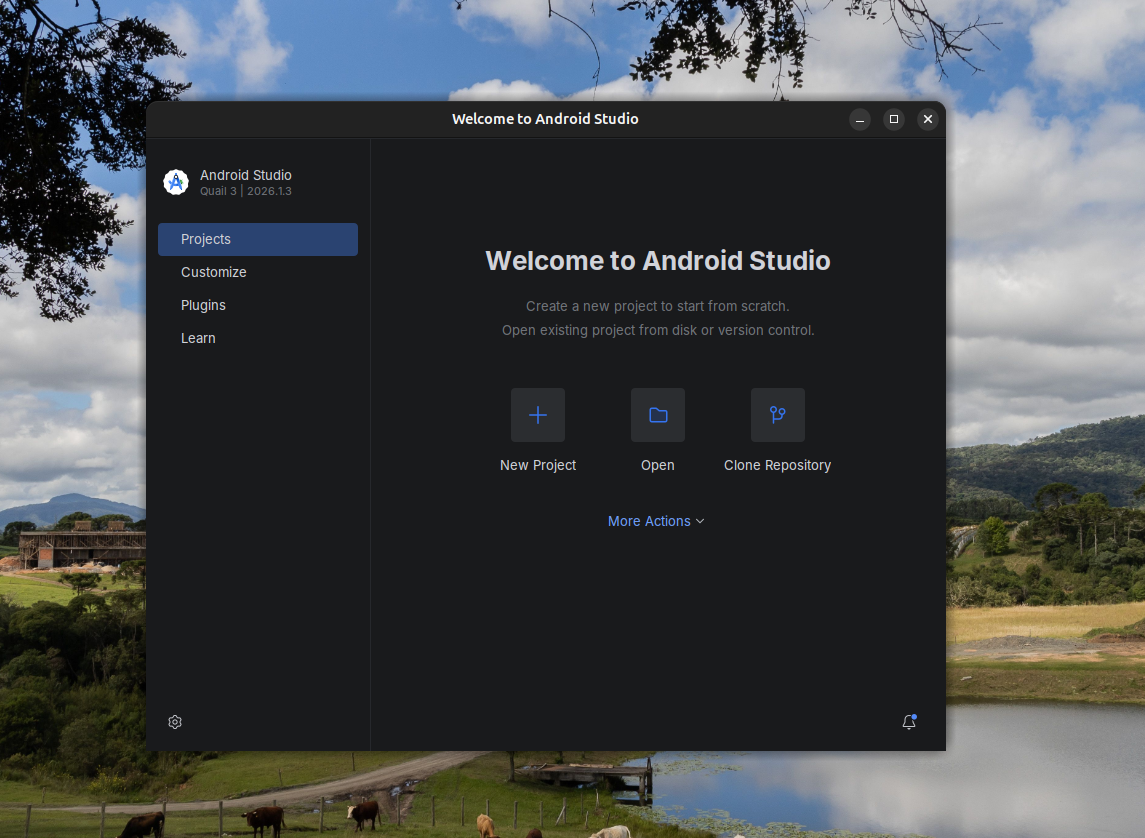
\includegraphics[width=\textwidth]{images/Captura de tela de 2026-08-10 15-22-47.png}
    \end{column}
  \end{columns}
\end{frame}

% -----------------------------------------------
% Seção: Criando um novo projeto
% -----------------------------------------------
\section{Criando um novo projeto}

\begin{frame}{Seleção do Template — Empty Activity}
  \begin{columns}[c]
    \begin{column}{0.45\textwidth}
      \begin{itemize}\small
        \item Na tela \textbf{New Project}, escolha a categoria \textbf{Phone and large screens}.
        \item Selecione o template \textbf{Empty Activity}.
        \item Este template cria um projeto com Jetpack Compose, a UI moderna do Android.
        \item Clique em \textbf{Next} para prosseguir.
      \end{itemize}
    \end{column}
    \begin{column}{0.52\textwidth}
      \centering
      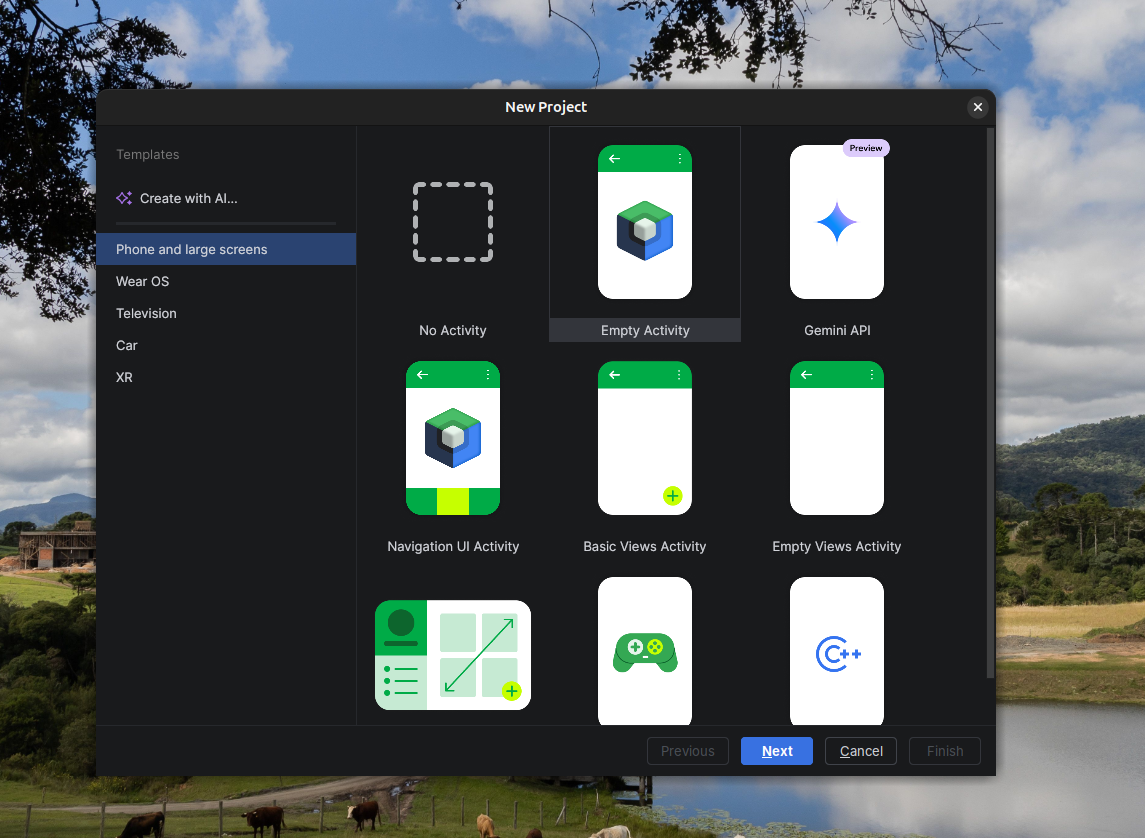
\includegraphics[width=\textwidth]{images/Captura de tela de 2026-08-10 15-23-00.png}
    \end{column}
  \end{columns}
\end{frame}

\begin{frame}{Seleção do Template — Empty Views Activity}
  \begin{columns}[c]
    \begin{column}{0.45\textwidth}
      \begin{itemize}\small
        \item Alternativamente, selecione \textbf{Empty Views Activity}.
        \item Usa o sistema de Views tradicional (XML + Kotlin).
        \item Ideal para aprender os fundamentos do Android.
        \item Outras opções incluem:
        \begin{itemize}\footnotesize
          \item Navigation UI Activity
          \item Basic Views Activity
          \item Gemini API (Preview)
        \end{itemize}
      \end{itemize}
    \end{column}
    \begin{column}{0.52\textwidth}
      \centering
      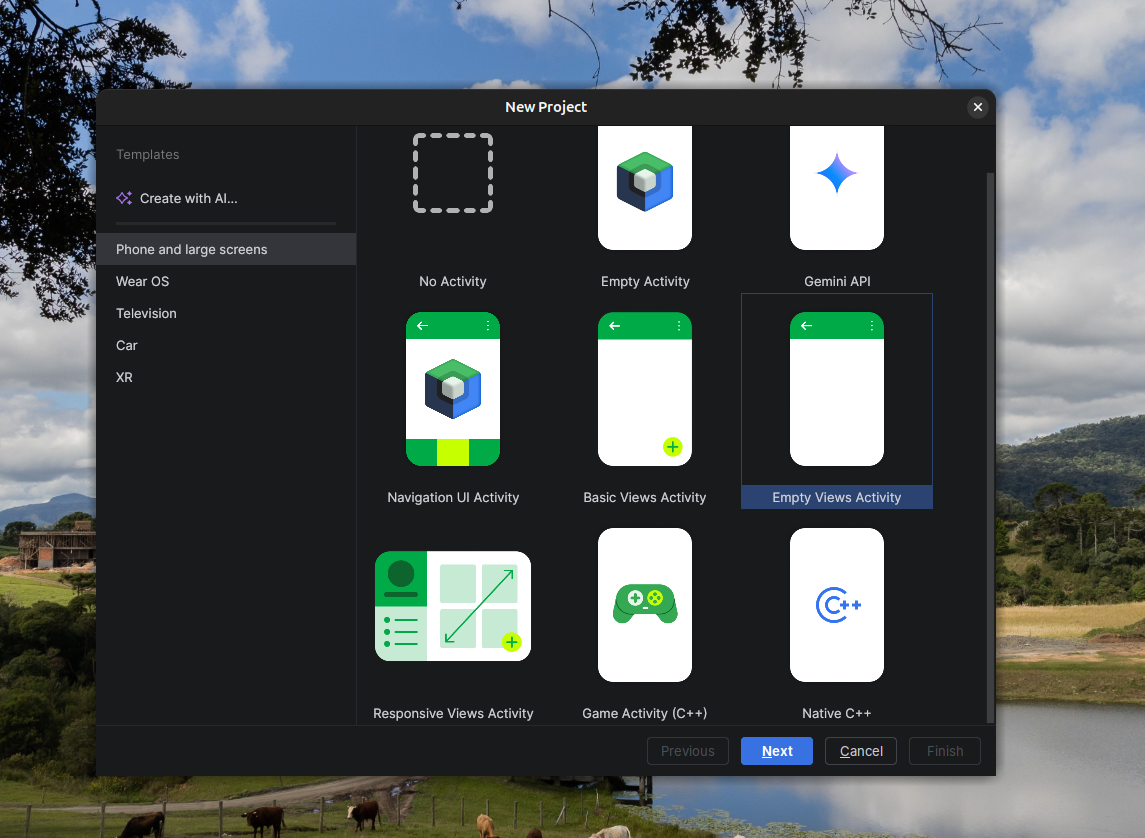
\includegraphics[width=\textwidth]{images/Captura de tela de 2026-08-10 15-23-39.png}
    \end{column}
  \end{columns}
\end{frame}

% -----------------------------------------------
% Seção: Configuração do Projeto
% -----------------------------------------------
\section{Configuração do Projeto}

\begin{frame}{Configuração do Projeto}
  \begin{columns}[c]
    \begin{column}{0.45\textwidth}
      \begin{itemize}\small
        \item \textbf{Name}: nome do app (ex: \texttt{PrimeiroProjeto}).
        \item \textbf{Package name}: identificador único (ex: \texttt{com.sergiosouzanovak.primeiroprojeto}).
        \item \textbf{Save location}: diretório onde o projeto será salvo.
        \item \textbf{Language}: selecione \textbf{Kotlin}.
        \item \textbf{Minimum SDK}: versão mínima do Android suportada (ex: API 26 — Android 8.0 Oreo).
        \item Clique em \textbf{Finish} para criar o projeto.
      \end{itemize}
    \end{column}
    \begin{column}{0.52\textwidth}
      \centering
      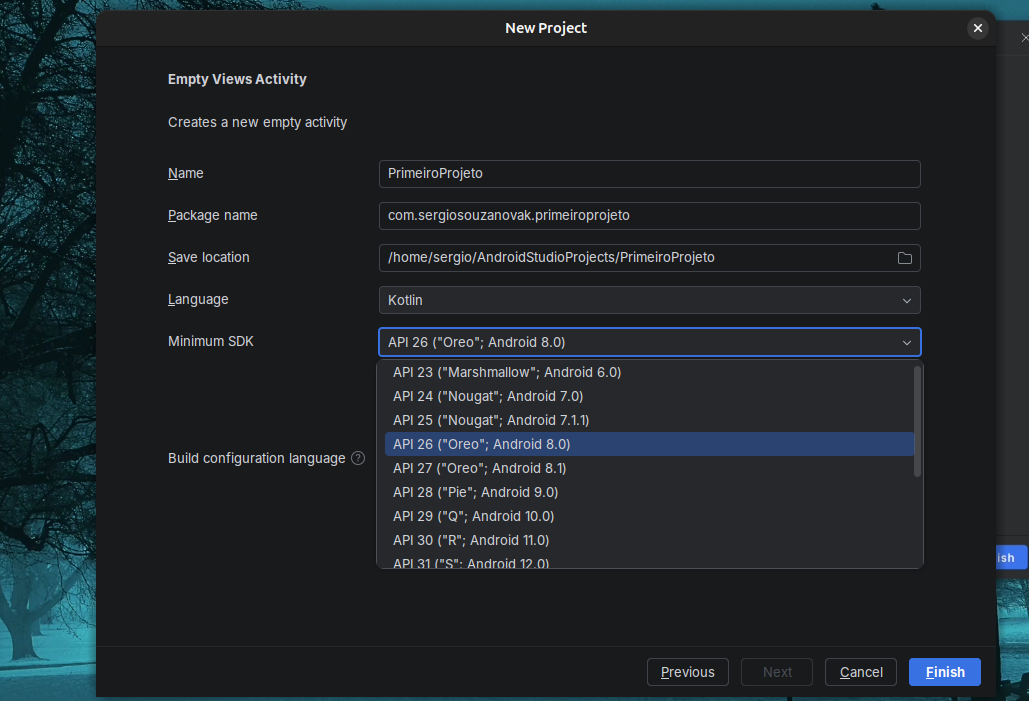
\includegraphics[width=\textwidth]{images/Captura de tela de 2026-08-10 15-28-46.png}
    \end{column}
  \end{columns}
\end{frame}

% -----------------------------------------------
% Seção: Estrutura do Projeto
% -----------------------------------------------
\section{Estrutura do Projeto}

\begin{frame}{Estrutura do Projeto — MainActivity.kt}
  \begin{columns}[c]
    \begin{column}{0.40\textwidth}
      \begin{itemize}\small
        \item O Android Studio abre o projeto e realiza o \textbf{Gradle Sync}.
        \item O arquivo \textbf{MainActivity.kt} é a Activity principal.
        \item Estrutura de pastas:
        \begin{itemize}\footnotesize
          \item \texttt{app/src/main/java/} — código Kotlin
          \item \texttt{app/src/main/res/} — recursos (layouts, strings, ícones)
          \item \texttt{build.gradle.kts} — configuração de build
        \end{itemize}
        \item A classe herda de \texttt{AppCompatActivity}.
      \end{itemize}
    \end{column}
    \begin{column}{0.58\textwidth}
      \centering
      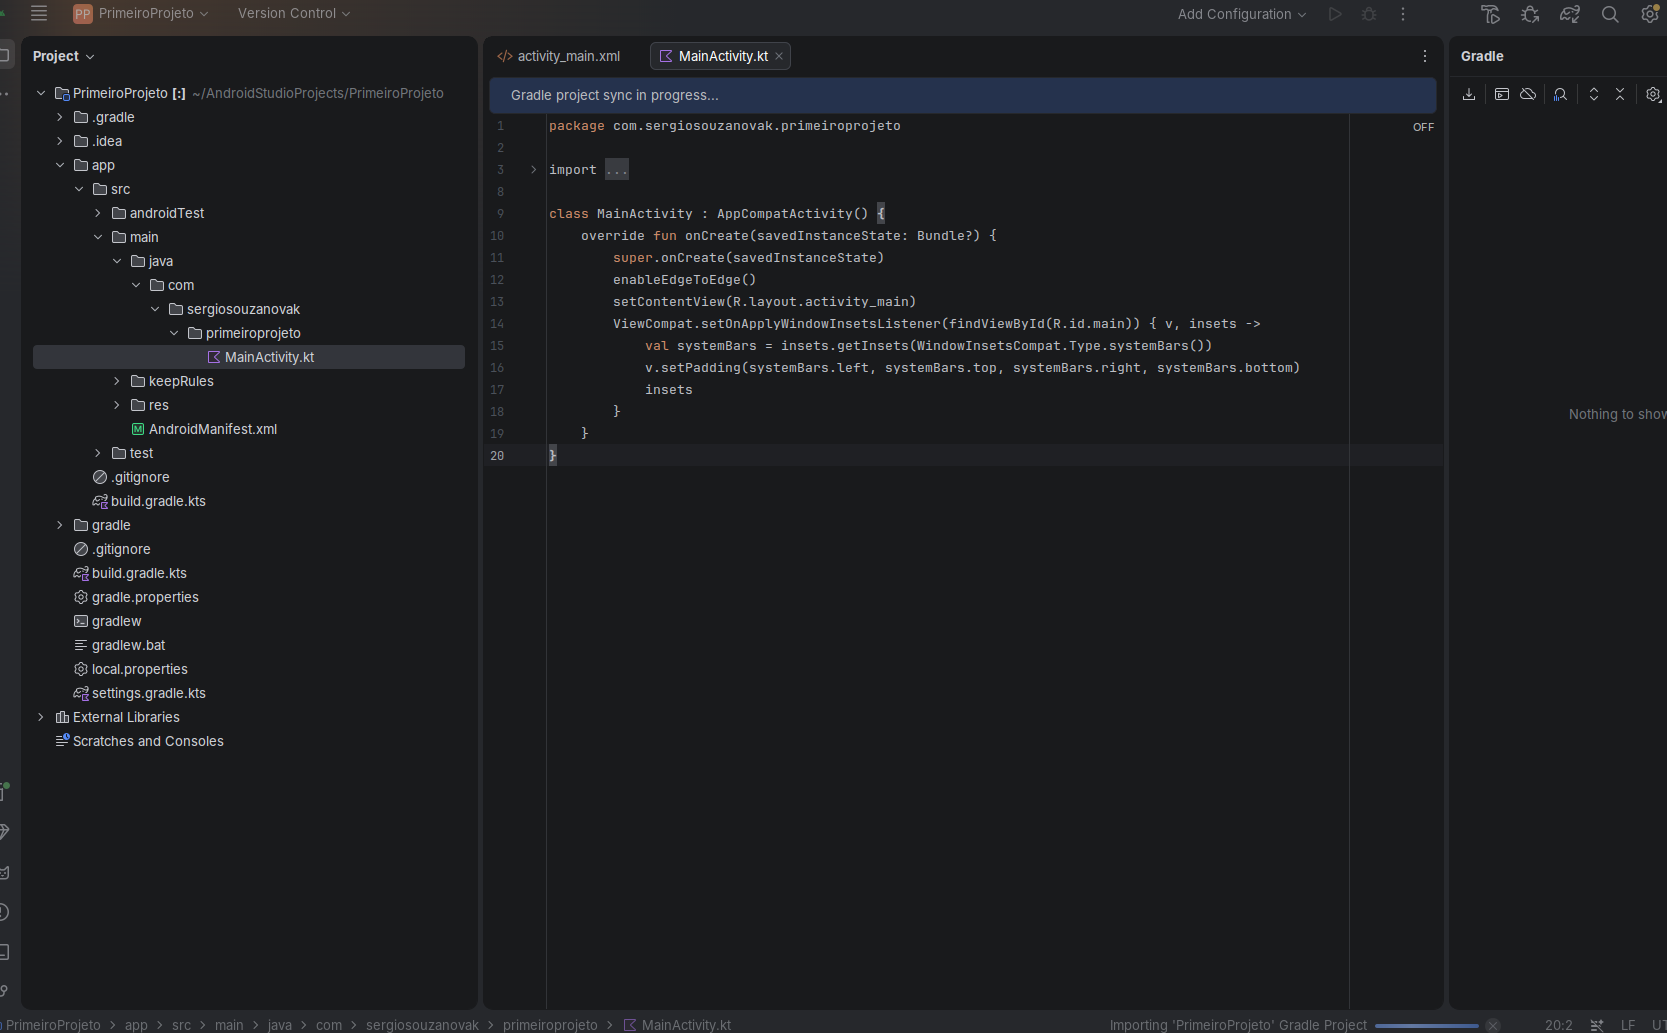
\includegraphics[width=\textwidth]{images/Captura de tela de 2026-08-10 15-31-28.png}
    \end{column}
  \end{columns}
\end{frame}

% -----------------------------------------------
% Seção: AndroidManifest.xml
% -----------------------------------------------
\section{AndroidManifest.xml}

\begin{frame}{AndroidManifest.xml}
  \begin{columns}[c]
    \begin{column}{0.40\textwidth}
      \begin{itemize}\small
        \item O \textbf{AndroidManifest.xml} descreve o app para o sistema Android.
        \item Contém:
        \begin{itemize}\footnotesize
          \item Nome do pacote
          \item Permissões
          \item Activities declaradas
          \item Ícone e tema do app
          \item Intent filters (qual Activity inicia o app)
        \end{itemize}
        \item A tag \texttt{<intent-filter>} com \texttt{MAIN} e \texttt{LAUNCHER} define o ponto de entrada.
      \end{itemize}
    \end{column}
    \begin{column}{0.58\textwidth}
      \centering
      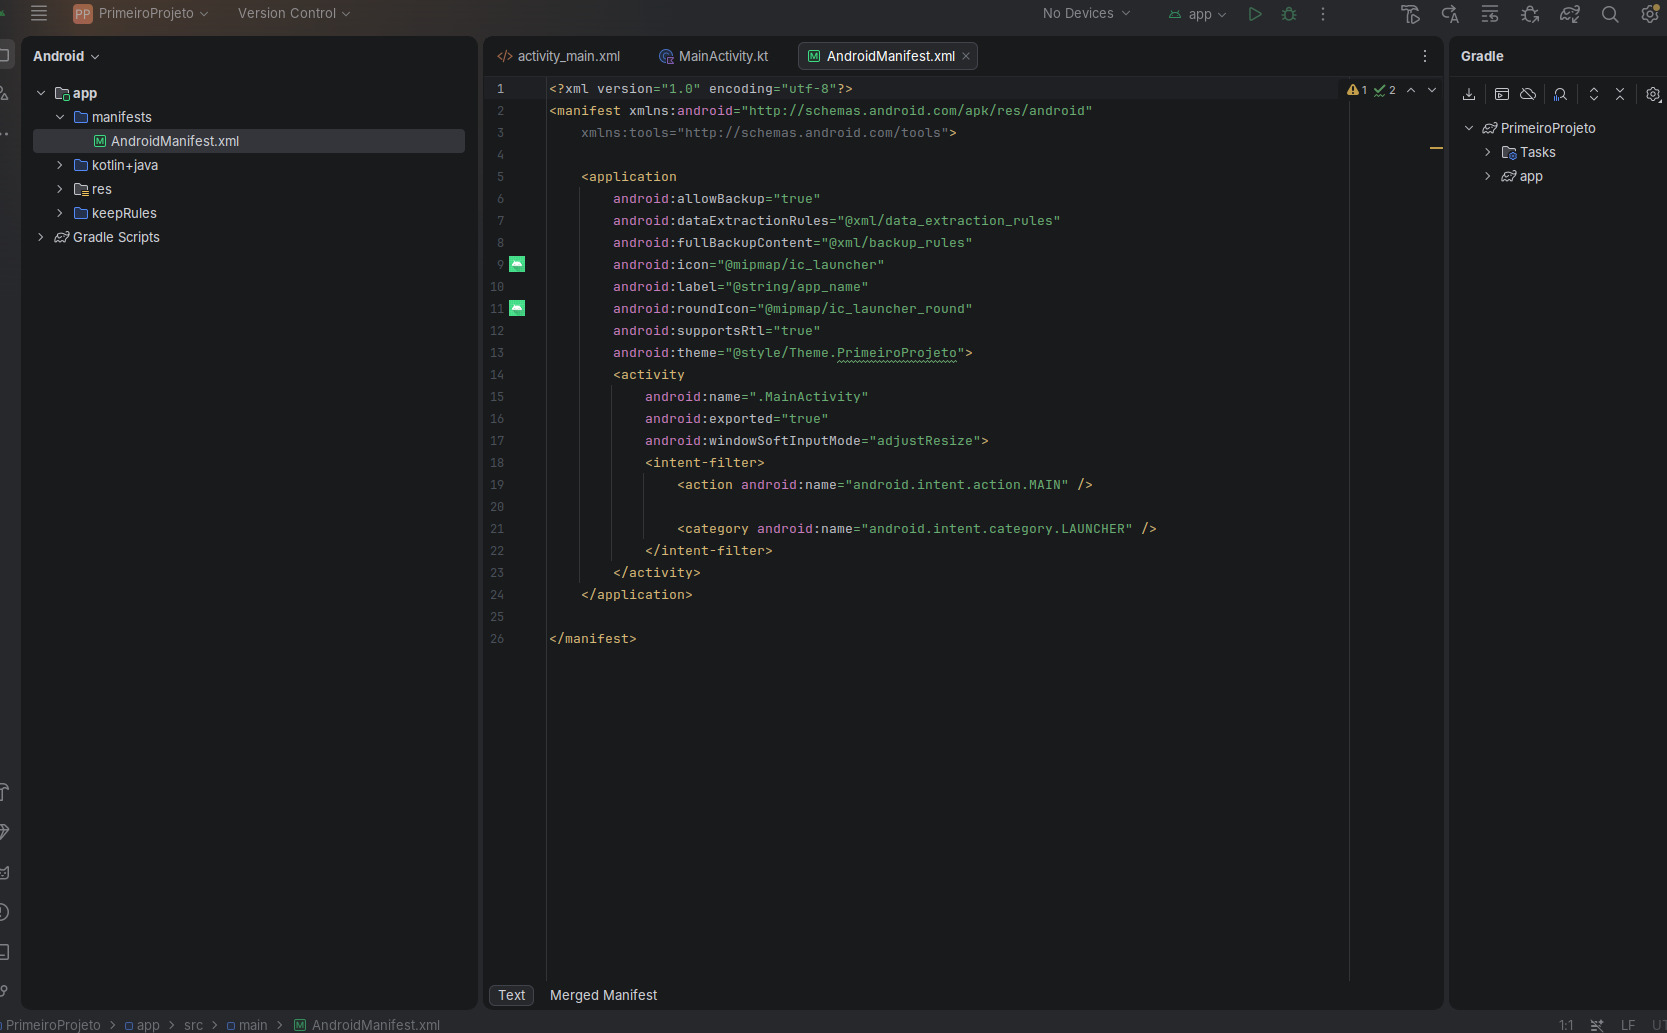
\includegraphics[width=\textwidth]{images/Captura de tela de 2026-08-10 15-34-17.png}
    \end{column}
  \end{columns}
\end{frame}
\begin{frame}[fragile]{AndroidManifest.xml}
\frametitle{AndroidManifest.xml}

O arquivo \texttt{AndroidManifest.xml} descreve informações essenciais
sobre o aplicativo Android.


\begin{block}{Estrutura básica}
  \scriptsize
\begin{verbatim}
<manifest>
    <application>
        <activity>
            <intent-filter>
                ...
            </intent-filter>
        </activity>
    </application>
</manifest>
\end{verbatim}
\end{block}

\begin{itemize}
    \item \textbf{manifest}: arquivo de configuração do aplicativo.
    \item \textbf{application}: configurações gerais do aplicativo.
    \item \textbf{activity}: define uma tela/atividade do aplicativo.
    \item \textbf{intent-filter}: define como a Activity pode ser iniciada.
\end{itemize}

\end{frame}
\begin{frame}[fragile]{AndroidManifest: \texttt{<application>}}
\small

O elemento \texttt{<application>} contém configurações globais do aplicativo.

\begin{block}{Exemplo}
    \tiny

\begin{verbatim}
<application
    android:allowBackup="true"
    android:dataExtractionRules="@xml/data_extraction_rules"
    android:fullBackupContent="@xml/backup_rules"
    android:icon="@mipmap/ic_launcher"
    android:label="@string/app_name"
    android:roundIcon="@mipmap/ic_launcher_round"
    android:supportsRtl="true"
    android:theme="@style/Theme.PrimeiroProjeto">
\end{verbatim}
\end{block}

\begin{description}
    \item[\texttt{allowBackup}] Permite recursos de backup do aplicativo.
    
    \item[\texttt{dataExtractionRules}] Define regras para extração/
    transferência de dados em versões recentes do Android.
    
    \item[\texttt{fullBackupContent}] Define regras de backup dos dados.
    
    \item[\texttt{icon}] Define o ícone principal do aplicativo.
    
    \item[\texttt{label}] Define o nome exibido para o aplicativo.
    
    \item[\texttt{roundIcon}] Define uma versão circular do ícone.
    
    \item[\texttt{supportsRtl}] Indica suporte à escrita da direita para a esquerda.
    
    \item[\texttt{theme}] Define o tema visual utilizado pelo aplicativo.
\end{description}

\end{frame}
\begin{frame}[fragile]{AndroidManifest: Activity e Intent}
\small

A \texttt{Activity} representa uma unidade de interação do aplicativo,
normalmente associada a uma tela.

\begin{block}{Activity principal}
\begin{verbatim}
<activity
    android:name=".MainActivity"
    android:exported="true"
    android:windowSoftInputMode="adjustResize">
\end{verbatim}
\end{block}

\begin{description}
    \item[\texttt{name}] Indica a classe da Activity.
    
    \item[\texttt{exported}] Indica se a Activity pode ser iniciada
    por componentes externos ao aplicativo.
    
    \item[\texttt{windowSoftInputMode}] Define como a janela deve
    se comportar quando o teclado virtual aparecer.
\end{description}

\vspace{0.2cm}

\begin{block}{Intent Filter}
    \scriptsize

\begin{verbatim}
<intent-filter>
    <action android:name="android.intent.action.MAIN" />
    <category android:name="android.intent.category.LAUNCHER" />
</intent-filter>
\end{verbatim}

\end{block}

\begin{itemize}
    \item \texttt{MAIN}: indica o ponto de entrada principal.
    \item \texttt{LAUNCHER}: permite que a Activity apareça
    como ponto de inicialização do aplicativo.
\end{itemize}

\end{frame}
\begin{frame}[fragile]{AndroidManifest: visão geral}

\begin{center}

\begin{tikzpicture}[
  scale=0.7,
    box/.style={
        draw,
        rounded corners,
        thick,
        align=center,
        minimum width=3cm,
        minimum height=0.9cm
    },
    arrow/.style={
        ->,
        thick
    }
]

\node[box] (manifest) at (0,0)
{\texttt{AndroidManifest.xml}\\
Configuração do aplicativo};

\node[box] (app) at (0,-1.7)
{\texttt{<application>}\\
Configurações gerais};

\node[box] (activity) at (0,-3.4)
{\texttt{<activity>}\\
Uma tela/Activity};

\node[box] (intent) at (0,-5.1)
{\texttt{<intent-filter>}\\
Como a Activity pode ser iniciada};

\draw[arrow] (manifest) -- (app);
\draw[arrow] (app) -- (activity);
\draw[arrow] (activity) -- (intent);

\end{tikzpicture}

\end{center}

\vspace{0.3cm}

\begin{alertblock}{No exemplo}
A sequência significa:

\centering
\textbf{Aplicativo}
$\rightarrow$
\textbf{MainActivity}
$\rightarrow$
\textbf{Ponto de entrada do aplicativo}
\end{alertblock}

\end{frame}

% -----------------------------------------------
% Seção: Estrutura Detalhada do Projeto
% -----------------------------------------------
\section{Estrutura Detalhada do Projeto}

\begin{frame}{Pacotes do Projeto (kotlin+java)}
  \begin{columns}[c]
    \begin{column}{0.55\textwidth}
      \begin{itemize}\small
        \item O código-fonte fica em \texttt{kotlin+java}.
        \item Três pacotes são criados automaticamente:
        \begin{itemize}\footnotesize
          \item \textbf{Pacote principal} — contém a \texttt{MainActivity} e o código do app.
          \item \textbf{androidTest} — testes de instrumentação (executados no dispositivo/emulador).
          \item \textbf{test} — testes unitários (executados na JVM local).
        \end{itemize}
        \item O nome do pacote segue a convenção: \texttt{com.empresa.app}.
      \end{itemize}
    \end{column}
    \begin{column}{0.42\textwidth}
      \centering
      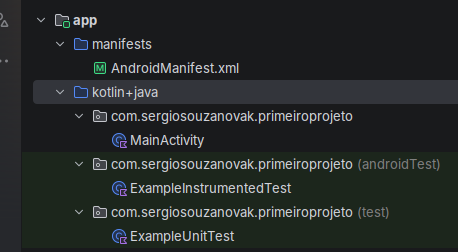
\includegraphics[width=\textwidth]{images/Captura de tela de 2026-08-10 15-53-57.png}
    \end{column}
  \end{columns}
\end{frame}

\begin{frame}{Pasta de Recursos (\texttt{res/})}
  \begin{columns}[c]
    \begin{column}{0.45\textwidth}
      \begin{itemize}\small
        \item A pasta \texttt{res/} contém todos os recursos do app:
        \begin{itemize}\footnotesize
          \item \textbf{drawable} — imagens e gráficos vetoriais (ícones).
          \item \textbf{layout} — arquivos XML de layout (\texttt{activity\_main.xml}).
          \item \textbf{mipmap} — ícones do app em várias resoluções.
          \item \textbf{values} — constantes: cores, strings, temas.
          \item \textbf{xml} — configurações de backup e extração de dados.
        \end{itemize}
      \end{itemize}
    \end{column}
    \begin{column}{0.52\textwidth}
      \centering
      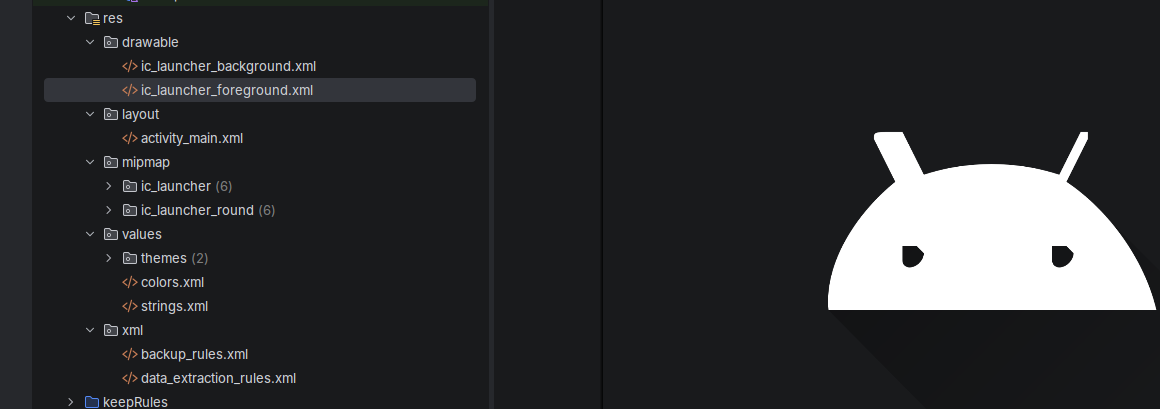
\includegraphics[width=\textwidth]{images/Captura de tela de 2026-08-10 15-55-34.png}
    \end{column}
  \end{columns}
\end{frame}

% -----------------------------------------------
% Seção: Layout XML
% -----------------------------------------------
\section{Layout XML}

\begin{frame}{Layout Editor — Modo Visual}
  \begin{columns}[c]
    \begin{column}{0.35\textwidth}
      \begin{itemize}\small
        \item O \textbf{Layout Editor} permite criar interfaces visualmente.
        \item Componentes disponíveis na \textbf{Palette}: Button, TextView, ImageView, etc.
        \item O \textbf{Component Tree} mostra a hierarquia de views.
        \item O painel \textbf{Attributes} permite configurar propriedades.
        \item Preview em tempo real do layout.
      \end{itemize}
    \end{column}
    \begin{column}{0.63\textwidth}
      \centering
      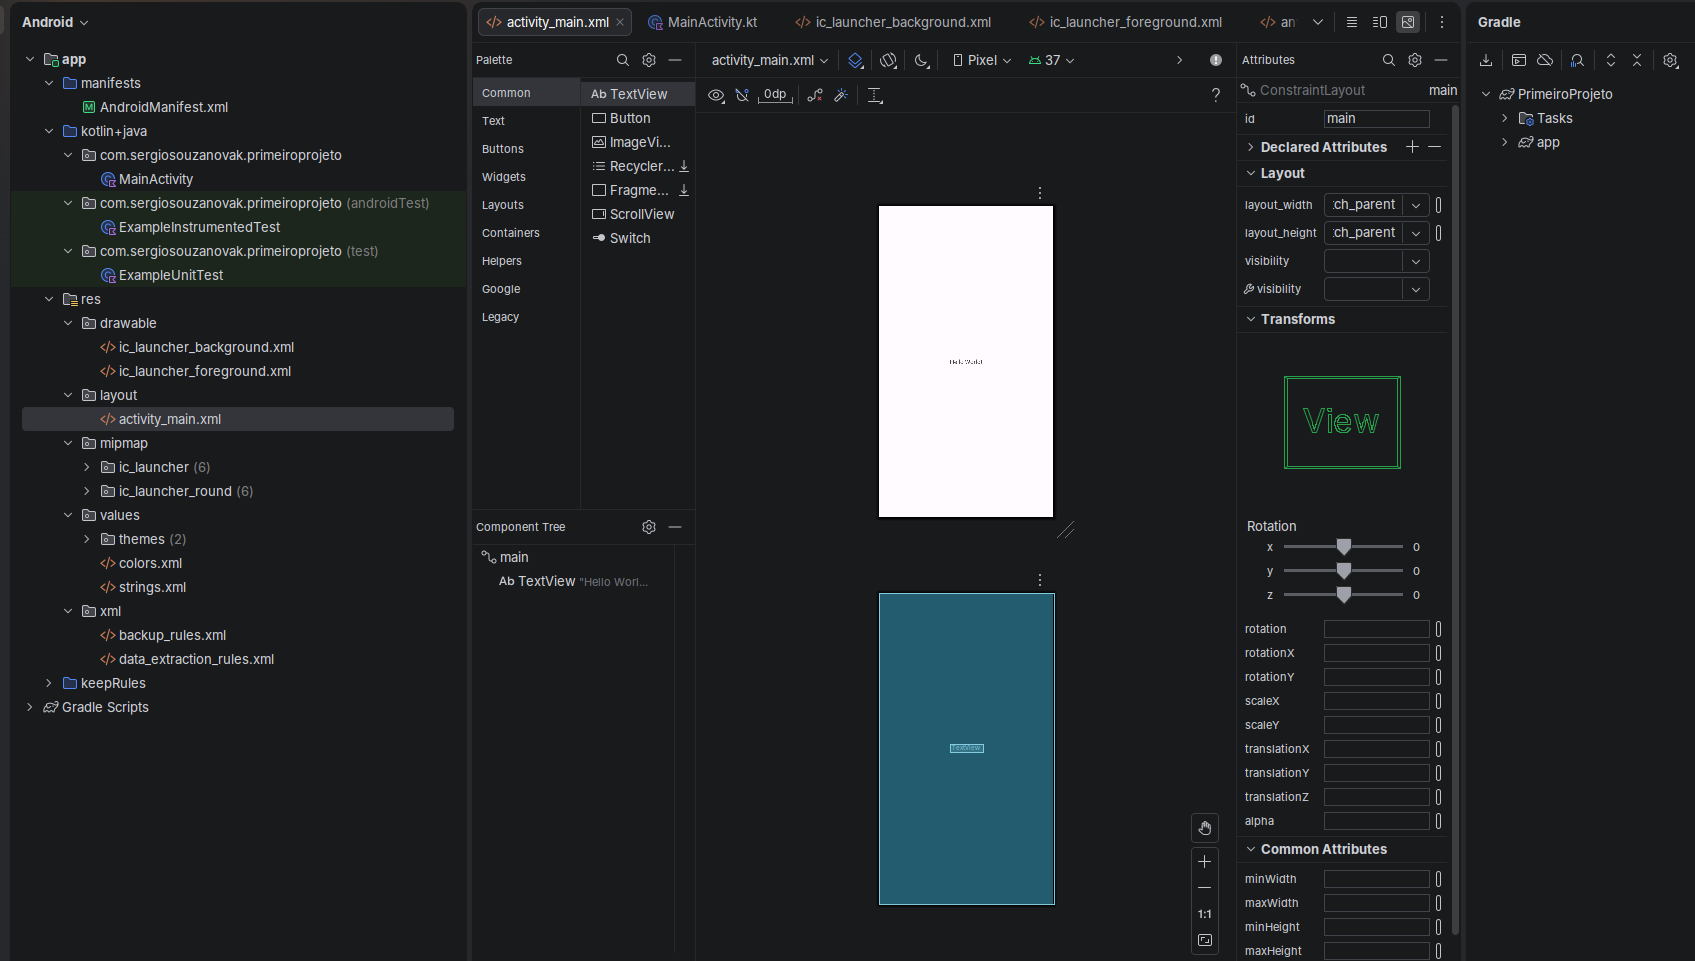
\includegraphics[width=\textwidth]{images/Captura de tela de 2026-08-10 15-56-53.png}
    \end{column}
  \end{columns}
\end{frame}

\begin{frame}{Layout XML — Modo Código}
  \begin{columns}[c]
    \begin{column}{0.35\textwidth}
      \begin{itemize}\small
        \item O arquivo \texttt{activity\_main.xml} define a interface.
        \item Usa \textbf{ConstraintLayout} como layout raiz.
        \item Contém um \textbf{TextView} com o texto ``Hello World!''.
        \item Constraints posicionam o TextView centralizado na tela.
        \item O preview é exibido ao lado do código XML.
      \end{itemize}
    \end{column}
    \begin{column}{0.63\textwidth}
      \centering
      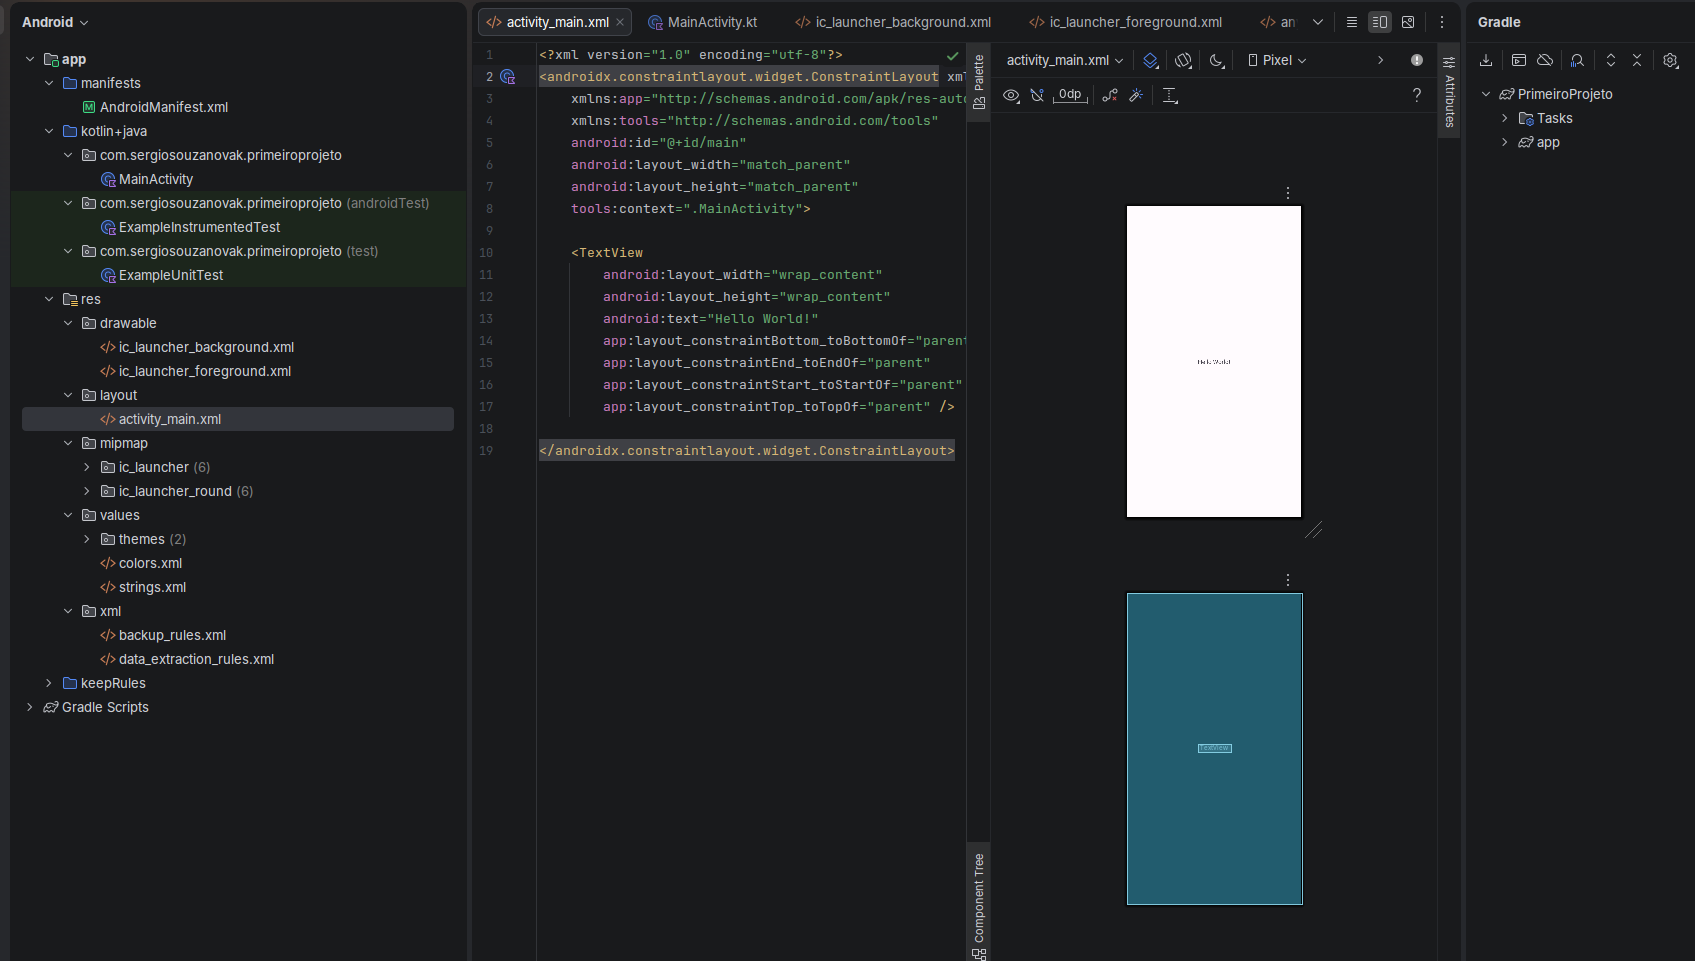
\includegraphics[width=\textwidth]{images/Captura de tela de 2026-08-10 15-57-20.png}
    \end{column}
  \end{columns}
\end{frame}

% -----------------------------------------------
% Seção: Recursos do Projeto
% -----------------------------------------------
\section{Recursos do Projeto}

\begin{frame}{Recursos: strings.xml e colors.xml}
  \begin{columns}[c]
    \begin{column}{0.48\textwidth}
      \centering
      \textbf{strings.xml}\\[0.3cm]
      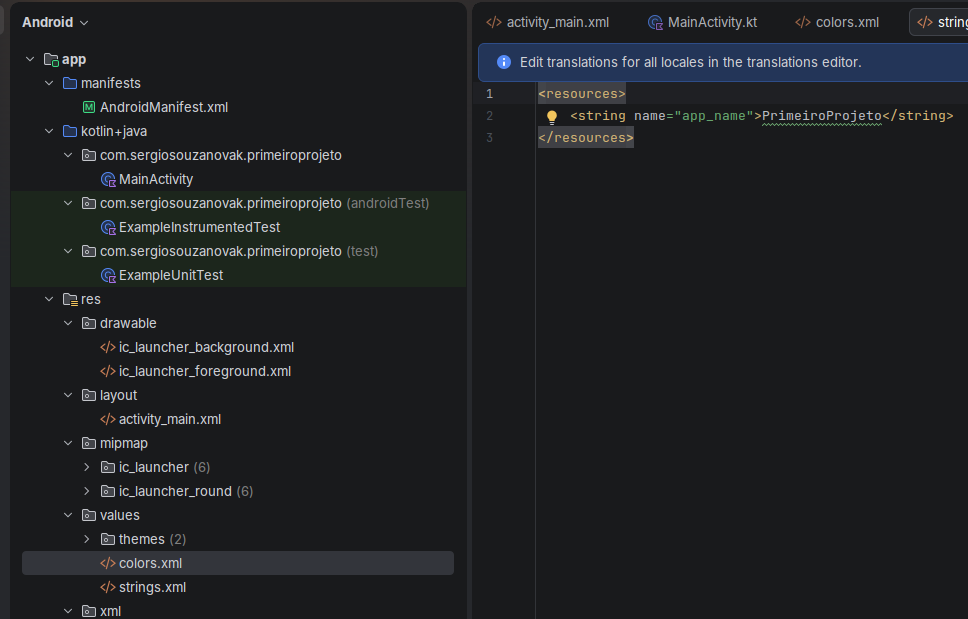
\includegraphics[width=\textwidth]{images/Captura de tela de 2026-08-10 15-59-20.png}
      \vspace{0.3cm}
      \begin{itemize}\scriptsize
        \item Define textos reutilizáveis do app.
        \item \texttt{app\_name}: nome exibido do aplicativo.
        \item Facilita a internacionalização (i18n).
      \end{itemize}
    \end{column}
    \begin{column}{0.48\textwidth}
      \centering
      \textbf{colors.xml}\\[0.3cm]
      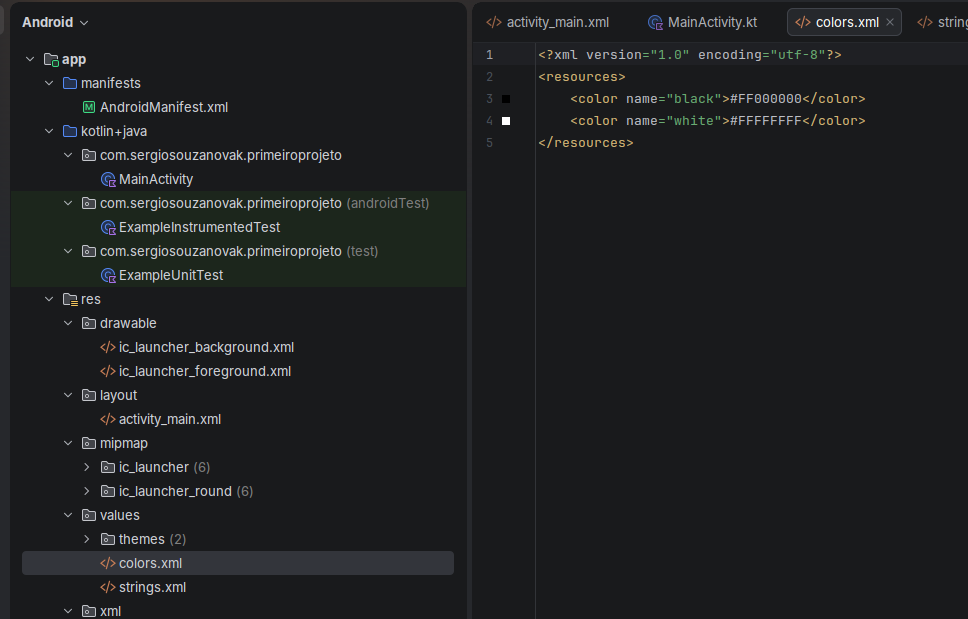
\includegraphics[width=\textwidth]{images/Captura de tela de 2026-08-10 15-59-30.png}
      \begin{itemize}\scriptsize
        \item Define as cores do app em formato hexadecimal.
        \item Cores padrão: \texttt{black} e \texttt{white}.
        \item Referenciadas como \texttt{@color/nome}.
      \end{itemize}
    \end{column}
  \end{columns}
\end{frame}


\begin{frame}{Recursos: themes.xml}
  \begin{columns}[c]
    \begin{column}{0.40\textwidth}
      \begin{itemize}\small
        \item O arquivo \texttt{themes.xml} define o tema visual do app.
        \item Herda de \textbf{Material3} (\texttt{Theme.Material3.DayNight.NoActionBar}).
        \item Permite personalizar cores primárias, secundárias, etc.
        \item Versão \textbf{night} para modo escuro (tema separado).
        \item O tema é referenciado no \texttt{AndroidManifest.xml}.
      \end{itemize}
    \end{column}
    \begin{column}{0.58\textwidth}
      \centering
      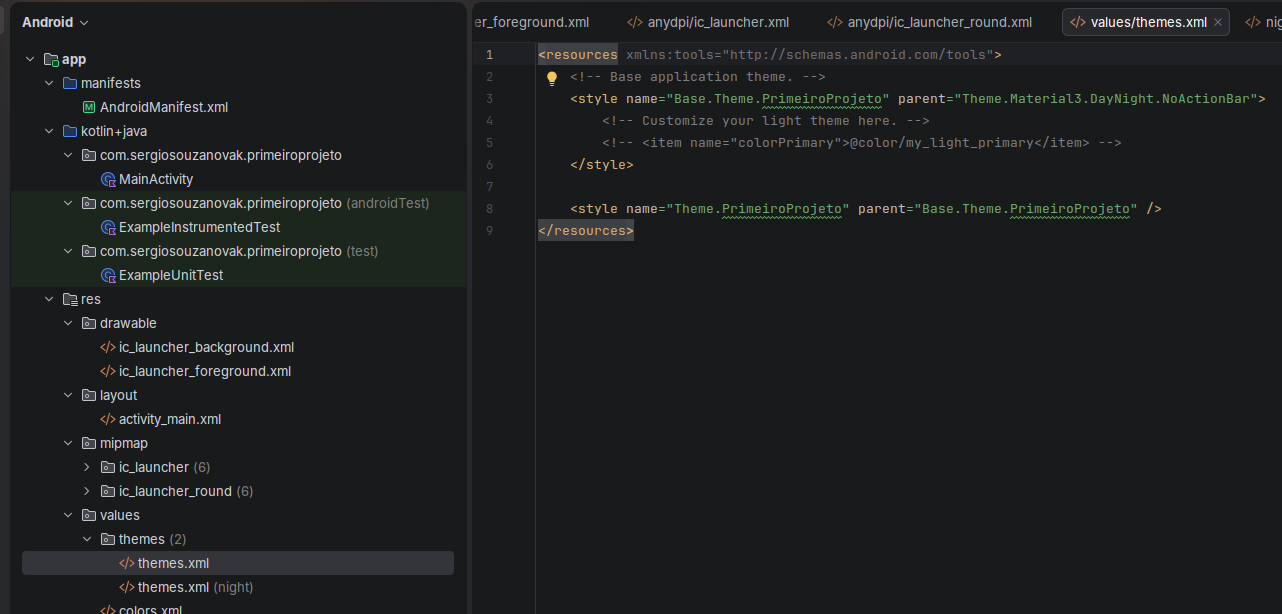
\includegraphics[width=\textwidth]{images/Captura de tela de 2026-08-10 16-00-44.png}
    \end{column}
  \end{columns}
\end{frame}

% -----------------------------------------------
% Seção: Build Gradle
% -----------------------------------------------
\section{Build Gradle}

\begin{frame}{build.gradle.kts — Configuração do Módulo}
  \begin{columns}[c]
    \begin{column}{0.35\textwidth}
      \begin{itemize}\small
        \item O \textbf{build.gradle.kts} (\texttt{:app}) configura o módulo.
        \item Seções principais:
        \begin{itemize}\footnotesize
          \item \textbf{plugins} — plugin Android
          \item \textbf{android} — SDK, namespace, versões
          \item \textbf{defaultConfig} — applicationId, minSdk, targetSdk
          \item \textbf{buildTypes} — configurações de release
          \item \textbf{compileOptions} — versão do Java
        \end{itemize}
      \end{itemize}
    \end{column}
    \begin{column}{0.63\textwidth}
      \centering
      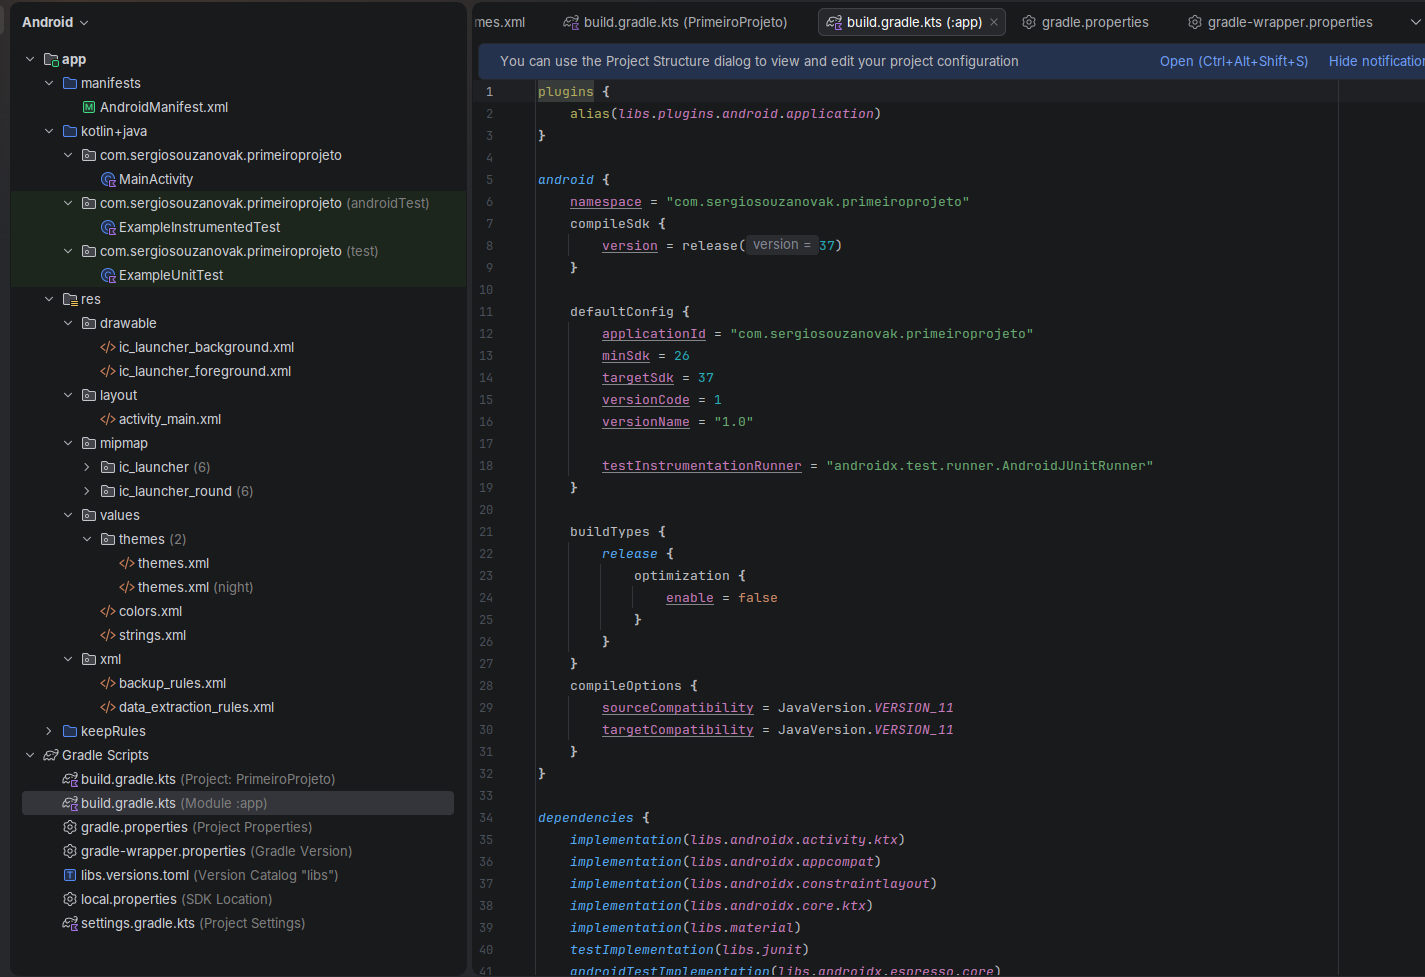
\includegraphics[width=\textwidth]{images/Captura de tela de 2026-08-10 16-02-44.png}
    \end{column}
  \end{columns}
\end{frame}

\begin{frame}{build.gradle.kts — Dependências}
  \begin{columns}[c]
    \begin{column}{0.40\textwidth}
      \begin{itemize}\small
        \item O bloco \textbf{dependencies} lista as bibliotecas utilizadas.
        \item Dependências padrão incluem:
        \begin{itemize}\footnotesize
          \item \texttt{activity.ktx} — extensões para Activity
          \item \texttt{appcompat} — compatibilidade
          \item \texttt{constraintlayout} — layout flexível
          \item \texttt{core.ktx} — extensões Kotlin
          \item \texttt{material} — Material Design
        \end{itemize}
        \item Testes: \texttt{junit}, \texttt{espresso}.
        \item Gerenciadas via \textbf{Version Catalog} (\texttt{libs.versions.toml}).
      \end{itemize}
    \end{column}
    \begin{column}{0.58\textwidth}
      \centering
      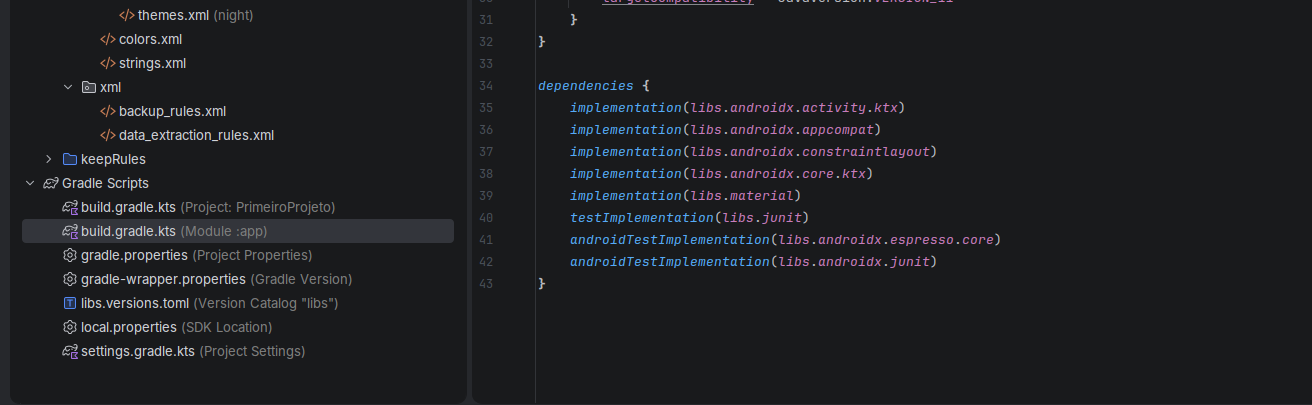
\includegraphics[width=\textwidth]{images/Captura de tela de 2026-08-10 16-03-06.png}
    \end{column}
  \end{columns}
\end{frame}

% -----------------------------------------------
% Seção: Executando o App
% -----------------------------------------------
\section{Executando o App}
\begin{frame}{Emulador Android}

\begin{center}
  \scriptsize
\begin{tikzpicture}[
    caixa/.style={
        draw,
        thick,
        rounded corners=4pt,
        align=center,
        minimum width=1cm,
        minimum height=1.2cm
    },
    seta/.style={
        ->,
        >=stealth,
        thick
    }
]

% Computador
\node[caixa] (pc) at (0,0)
{
    \textbf{Computador}\\
    Ubuntu / Windows / macOS\\
    CPU + RAM + GPU
};

% Emulador
\node[caixa] (emulador) at (5,0)
{
    \textbf{Emulador Android}\\
    Dispositivo virtual\\
    Android
};

% Aplicativo
\node[caixa] (app) at (10,0)
{
    \textbf{Aplicativo}\\
    APK / App em execução\\
    $\mathrm{MainActivity}$
};

% Setas
\draw[seta] (pc) -- node[above, font=\small]{executa} (emulador);
\draw[seta] (emulador) -- node[above, font=\small]{executa} (app);

% Recursos simulados
\node[caixa, minimum width=4cm] (recursos) at (5,-2.5)
{
    \textbf{Recursos simulados}\\
    Tela \quad GPS \quad Câmera\\
    Sensores \quad Rede \quad Armazenamento
};

\draw[seta] (emulador) -- (recursos);

\end{tikzpicture}
\end{center}

\vspace{0.2cm}

\begin{block}{Definição}
O \textbf{emulador Android} é um software que simula um dispositivo
Android dentro do computador, permitindo desenvolver e testar
aplicativos sem utilizar um dispositivo físico.
\end{block}

\end{frame}
\begin{frame}{Configurando o Emulador — SDK e Device Manager}
  \begin{columns}[c]
    \begin{column}{0.40\textwidth}
      \begin{itemize}\small
        \item Antes de executar, é necessário instalar a \textbf{System Image} do Android.
        \item O Android Studio baixa automaticamente via \textbf{SDK Component Installer}.
        \item Após a instalação, o \textbf{Device Manager} exibe os dispositivos virtuais.
        \item No exemplo: \textbf{Small Phone} com API 37.1 (Android 17.0).
      \end{itemize}
    \end{column}
    \begin{column}{0.58\textwidth}
      \centering
      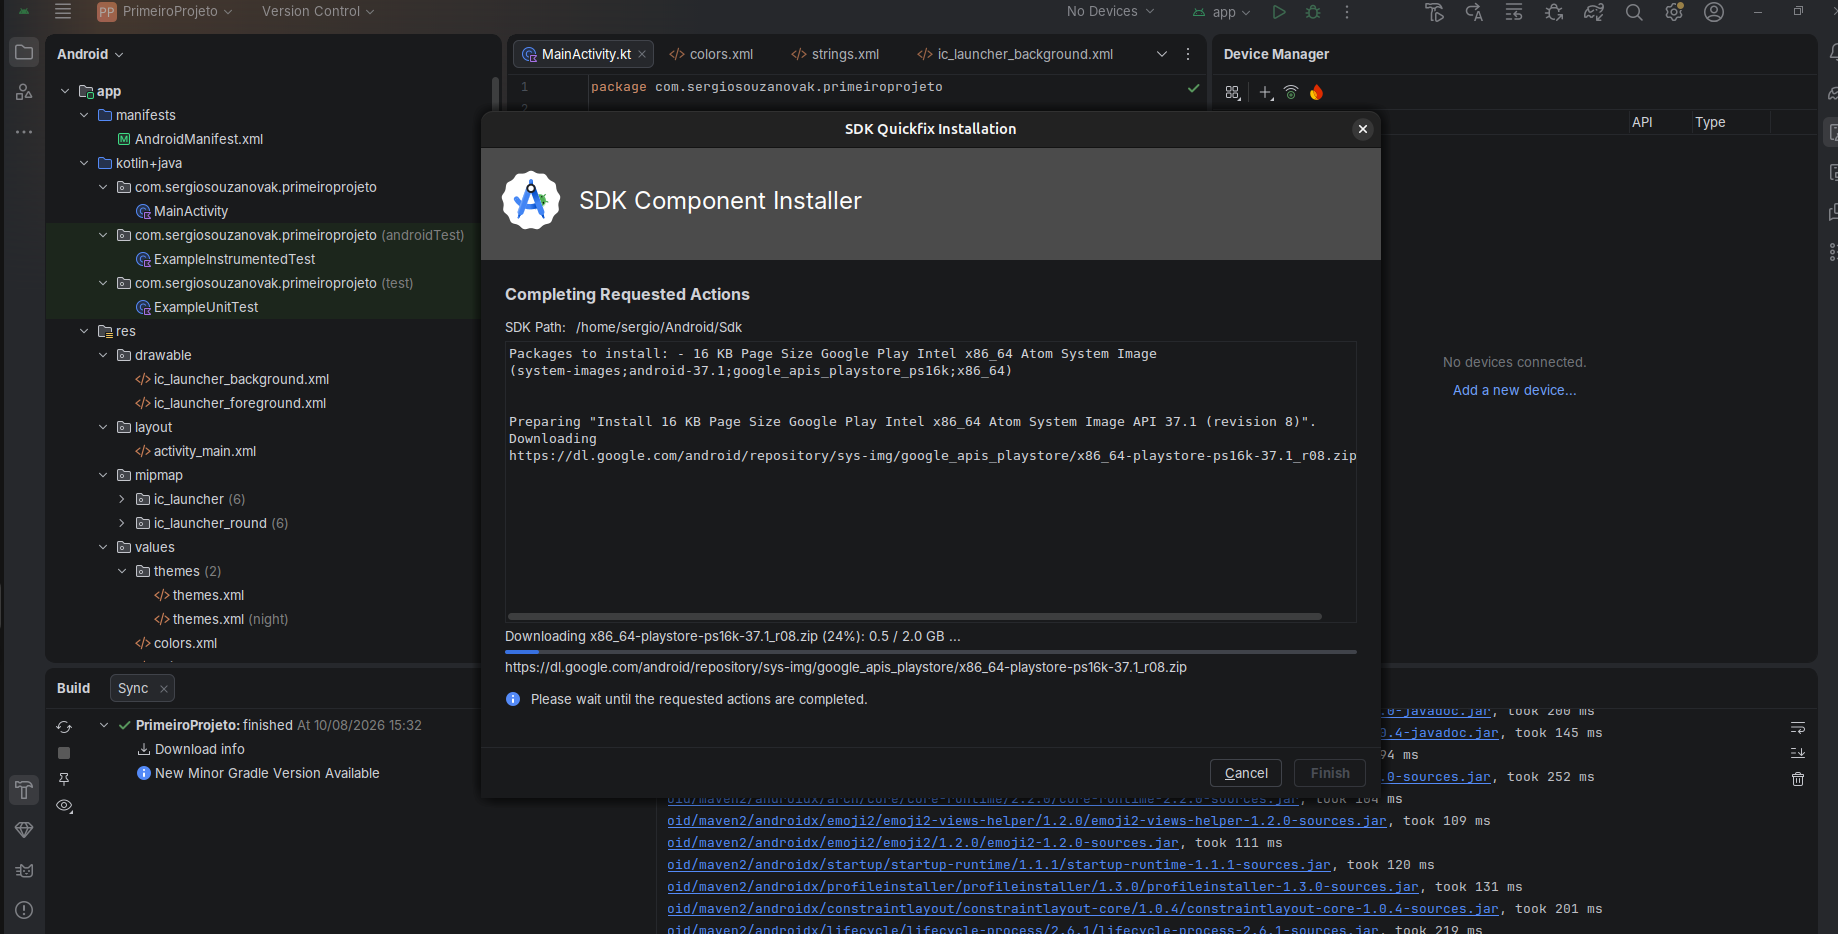
\includegraphics[width=0.95\textwidth]{images/Captura de tela de 2026-08-10 16-06-12.png}
      \vspace{0.2cm}
      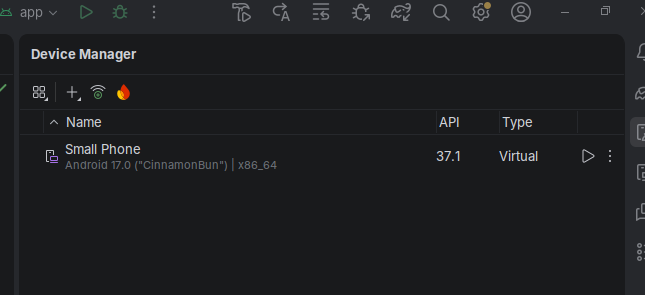
\includegraphics[width=0.7\textwidth]{images/Captura de tela de 2026-08-10 16-10-43.png}
    \end{column}
  \end{columns}
\end{frame}

\begin{frame}{Executando o App — Hello World!}
  \begin{columns}[c]
    \begin{column}{0.35\textwidth}
      \begin{itemize}\small
        \item Clique no botão \textbf{Run}, ou aperte play, ou pressione \texttt{Shift+F10}.
        \item O Android Studio compila o app e inicia o emulador.
        \item O app é instalado e executado automaticamente.
        \item Resultado: a tela exibe ``\textbf{Hello World!}'' centralizado.
        \item O primeiro app Kotlin está funcionando!
      \end{itemize}
    \end{column}
    \begin{column}{0.63\textwidth}
      \centering
      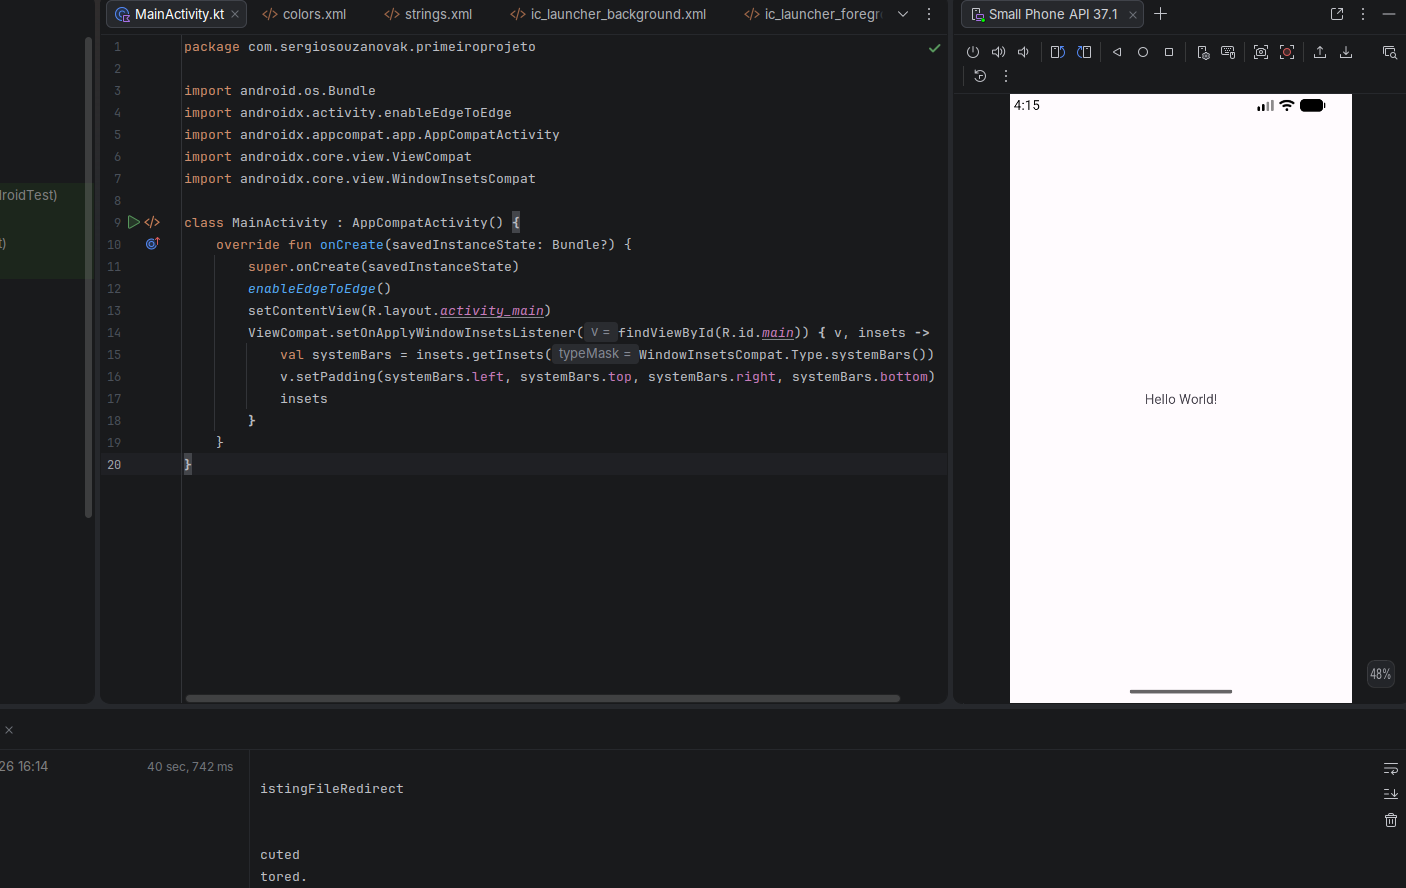
\includegraphics[width=\textwidth]{images/Captura de tela de 2026-08-10 16-15-12.png}
    \end{column}
  \end{columns}
\end{frame}

% -----------------------------------------------
% Seção: Código Android — Explicação Detalhada
% -----------------------------------------------
\section{Código Android — Explicação Detalhada}

\begin{frame}[fragile]{Código Android: \texttt{package}}

\begin{block}{Primeira linha}
\begin{verbatim}
package com.sergiosouzanovak.primeiroprojeto
\end{verbatim}
\end{block}

\vspace{0.3cm}
\scriptsize

\begin{tikzpicture}[
    parte/.style={
        draw,
        thick,
        rounded corners=4pt,
        align=center,
        minimum height=1cm
    },
    seta/.style={
        ->,
        >=stealth,
        thick
    }
]

\node[parte] (com) at (0,0)
{\texttt{com}\\
Domínio};

\node[parte] (autor) at (3,0)
{\texttt{sergiosouzanovak}\\
Desenvolvedor/organização};

\node[parte] (projeto) at (6.5,0)
{\texttt{primeiroprojeto}\\
Aplicação};

\draw[seta] (com) -- (autor);
\draw[seta] (autor) -- (projeto);

\end{tikzpicture}

\vspace{0.4cm}

\begin{itemize}
    \item Define o \textbf{pacote} ao qual a classe pertence.
    \item Organiza as classes e recursos do projeto.
    \item Ajuda a evitar conflitos de nomes entre aplicativos.
    \item É utilizado pelo Android para identificar o código da aplicação.
\end{itemize}

\begin{alertblock}{Exemplo}
O pacote funciona como o ``endereço'' da classe dentro do projeto.
\end{alertblock}

\end{frame}

\begin{frame}[fragile]{Código Android: \texttt{import}}

O comando \texttt{import} permite utilizar classes e funções
disponíveis em outras bibliotecas.

\begin{block}{Imports do projeto}
\begin{verbatim}
import android.os.Bundle

import androidx.activity.enableEdgeToEdge
import androidx.appcompat.app.AppCompatActivity
import androidx.core.view.ViewCompat
import androidx.core.view.WindowInsetsCompat
\end{verbatim}
\end{block}

\vspace{0.3cm}

\begin{tikzpicture}[
    biblioteca/.style={
        draw,
        thick,
        rounded corners=4pt,
        align=center,
        minimum width=3.4cm,
        minimum height=1cm
    },
    seta/.style={
        ->,
        >=stealth,
        thick
    }
]

\node[biblioteca] (android) at (0,0)
{\textbf{Android}\\
\texttt{Bundle}};

\node[biblioteca] (activity) at (4,0)
{\textbf{AndroidX Activity}\\
\texttt{AppCompatActivity}};

\node[biblioteca] (view) at (8,0)
{\textbf{AndroidX Core}\\
\texttt{ViewCompat}};

\node[biblioteca] (window) at (4,-1.8)
{\texttt{WindowInsetsCompat}\\
Barras do sistema};

\draw[seta] (android) -- (activity);
\draw[seta] (activity) -- (view);
\draw[seta] (view) -- (window);

\end{tikzpicture}

\end{frame}

\begin{frame}[fragile]{Código Android: \texttt{MainActivity}}

\begin{block}{Declaração da classe}
\begin{verbatim}
class MainActivity : AppCompatActivity() {
    ...
}
\end{verbatim}
\end{block}

\vspace{0.3cm}
\scriptsize
\begin{tikzpicture}[
    caixa/.style={
        draw,
        thick,
        rounded corners=5pt,
        align=center,
        minimum width=2cm,
        minimum height=1.1cm
    },
    seta/.style={
        ->,
        >=stealth,
        thick
    }
]

\node[caixa] (app) at (0,0)
{\textbf{AppCompatActivity}\\
Classe da biblioteca AndroidX};

\node[caixa] (main) at (0,-2)
{\textbf{MainActivity}\\
Tela principal do aplicativo};

\draw[seta] (app) -- node[right]{herança} (main);

\end{tikzpicture}

\vspace{0.3cm}

\begin{itemize}
    \item \texttt{class}: declara uma classe Kotlin.
    \item \texttt{MainActivity}: nome da classe.
    \item \texttt{: AppCompatActivity()}: indica \textbf{herança}.
    \item A Activity representa uma tela/interação do aplicativo.
\end{itemize}

\begin{alertblock}{Conceito importante}
\texttt{MainActivity} herda funcionalidades de
\texttt{AppCompatActivity}.
\end{alertblock}

\end{frame}

\begin{frame}[fragile]{Código Android: \texttt{onCreate()}}

\begin{block}{Método de inicialização}
\begin{verbatim}
override fun onCreate(savedInstanceState: Bundle?) {
    super.onCreate(savedInstanceState)
    enableEdgeToEdge()
    setContentView(R.layout.activity_main)
}
\end{verbatim}
\end{block}

\vspace{0.2cm}
\scriptsize
\begin{tikzpicture}[
    etapa/.style={
        draw,
        thick,
        rounded corners=5pt,
        align=center,
        minimum width=3.5cm,
        minimum height=1.1cm
    },
    seta/.style={
        ->,
        >=stealth,
        thick
    }
]

\node[etapa] (inicio) at (0,0)
{\texttt{onCreate()}\\
Activity criada};

\node[etapa] (super) at (4.5,0)
{\texttt{super.onCreate()}\\
Inicialização da Activity};

\node[etapa] (edge) at (9,0)
{\texttt{enableEdgeToEdge()}\\
Conteúdo até as bordas};

\node[etapa] (layout) at (4.5,-2)
{\texttt{setContentView()}\\
Carrega a interface};

\draw[seta] (inicio) -- (super);
\draw[seta] (super) -- (edge);
\draw[seta] (edge) -- (layout);

\end{tikzpicture}

\vspace{0.3cm}

\begin{itemize}
    \item \texttt{override}: sobrescreve um método da classe pai.
    \item \texttt{onCreate()}: executado quando a Activity é criada.
    \item \texttt{savedInstanceState}: pode armazenar o estado anterior da Activity.
    \item \texttt{setContentView()}: associa a Activity ao layout XML.
\end{itemize}

\end{frame}

\begin{frame}[fragile]{\texttt{setContentView()} e o layout XML}

\begin{block}{Código Kotlin}
\begin{verbatim}
setContentView(R.layout.activity_main)
\end{verbatim}
\end{block}

\vspace{0.2cm}
\scriptsize
\begin{tikzpicture}[
    caixa/.style={
        draw,
        thick,
        rounded corners=5pt,
        align=center,
        minimum width=3cm,
        minimum height=1.2cm
    },
    seta/.style={
        ->,
        >=stealth,
        thick
    }
]

\node[caixa] (kotlin) at (-1,0)
{
    \textbf{MainActivity.kt}\\
    Código Kotlin
};

\node[caixa] (resource) at (6,0)
{
    \textbf{R}\\
    Classe de recursos
};

\node[caixa] (xml) at (11,0)
{
    \textbf{activity\_main.xml}\\
    Interface gráfica
};

\draw[seta] (kotlin) --
node[above]{\texttt{R.layout.activity\_main}}
(resource);

\draw[seta] (resource) --
node[above]{referencia}
(xml);

\end{tikzpicture}

\vspace{0.5cm}

\begin{itemize}
    \item \texttt{R} é uma classe gerada automaticamente pelo Android.
    \item \texttt{layout} representa a pasta de layouts.
    \item \texttt{activity\_main} identifica o arquivo XML.
    \item O XML define a interface visual.
    \item O Kotlin controla o comportamento da interface.
\end{itemize}

\begin{alertblock}{Resumo}
\centering
\textbf{Kotlin = comportamento}
\qquad
\textbf{XML = interface}
\end{alertblock}

\end{frame}

\begin{frame}[fragile]{Conteúdo e barras do sistema}

\begin{block}{Código}
  \scriptsize
\begin{verbatim}
enableEdgeToEdge()

ViewCompat.setOnApplyWindowInsetsListener(
    findViewById(R.id.main)
) { v, insets ->

    val systemBars =
        insets.getInsets(
            WindowInsetsCompat.Type.systemBars()
        )

    v.setPadding(
        systemBars.left,
        systemBars.top,
        systemBars.right,
        systemBars.bottom
    )

    insets
}
\end{verbatim}
\end{block}

\begin{tikzpicture}[
    caixa/.style={
        draw,
        thick,
        rounded corners=4pt,
        align=center,
        minimum width=3.5cm,
        minimum height=0.9cm
    },
    seta/.style={
        ->,
        >=stealth,
        thick
    }
]

\node[caixa] (app) at (0,0)
{\textbf{Aplicativo}\\
Conteúdo};

\node[caixa] (bars) at (5,0)
{\textbf{Barras do sistema}\\
Status + Navegação};

\node[caixa] (padding) at (10,0)
{\textbf{Padding}\\
Espaço de segurança};

\draw[seta] (app) --
node[above]{\texttt{WindowInsetsCompat}} (bars);

\draw[seta] (bars) --
node[above]{dimensões} (padding);

\end{tikzpicture}

\vspace{0.3cm}

\begin{itemize}
    \item \texttt{enableEdgeToEdge()}: permite que o conteúdo ocupe toda a tela.
    \item \texttt{WindowInsetsCompat}: informa o espaço ocupado pelas barras do sistema.
    \item \texttt{setPadding()}: adiciona espaçamento para evitar sobreposição.
\end{itemize}

\end{frame}

\begin{frame}{MainActivity: fluxo de execução}

\begin{center}

\begin{tikzpicture}[
    etapa/.style={
        draw,
        thick,
        rounded corners=5pt,
        align=center,
        minimum width=3.3cm,
        minimum height=1cm
    },
    seta/.style={
        ->,
        >=stealth,
        very thick
    }
]

\node[etapa] (package) at (0,0)
{\textbf{package}\\
Define o pacote};

\node[etapa] (imports) at (4,0)
{\textbf{import}\\
Importa bibliotecas};

\node[etapa] (class) at (8,0)
{\textbf{MainActivity}\\
Define a Activity};

\node[etapa] (create) at (8,-2)
{\textbf{onCreate()}\\
Inicializa a tela};

\node[etapa] (layout) at (4,-2)
{\textbf{setContentView()}\\
Carrega o XML};

\node[etapa] (insets) at (0,-2)
{\textbf{WindowInsets}\\
Ajusta a interface};

\draw[seta] (package) -- (imports);
\draw[seta] (imports) -- (class);
\draw[seta] (class) -- (create);
\draw[seta] (create) -- (layout);
\draw[seta] (layout) -- (insets);

\end{tikzpicture}

\end{center}

\vspace{0.3cm}

\begin{alertblock}{Em resumo}
\centering
\texttt{MainActivity.kt} é responsável por inicializar a Activity,
carregar a interface e configurar o comportamento da tela.
\end{alertblock}

\end{frame}
\begin{frame}{Conceitos iniciais}

% ------------------------------------------------
% Primeiro tópico
% ------------------------------------------------

\begin{tikzpicture}[
    every node/.style={font=\normalsize}
]

\node[
    circle,
    fill=meuazul,
    minimum size=0.25cm,
    inner sep=0pt
] at (0.15,0)
{};

\node[
    anchor=west,
    font=\bfseries
] at (0.45,0)
{Define a estrutura da interface gráfica};

\node[
    circle,
    draw=meuazul,
    thick,
    minimum size=0.18cm,
    inner sep=0pt
] at (0.65,-0.65)
{};

\node[
    anchor=west
] at (0.95,-0.65)
{Como os elementos se comportam e se relacionam};

% ------------------------------------------------
% Segundo tópico
% ------------------------------------------------

\node[
    circle,
    fill=meuazul,
    minimum size=0.25cm,
    inner sep=0pt
] at (0.15,-1.55)
{};

\node[
    anchor=west,
    font=\bfseries
] at (0.45,-1.55)
{Todos os elementos dentro do layout respeitam a hierarquia de
View e ViewGroup};

\end{tikzpicture}

\vspace{0.25cm}

% ------------------------------------------------
% Quadros View e ViewGroup
% ------------------------------------------------

\begin{tikzpicture}[
    quadro/.style={
        draw=meuazul,
        thick,
        rounded corners=4pt,
        minimum width=7cm,
        minimum height=3.7cm,
        align=center
    },
    titulo/.style={
        fill=meuazul,
        text=white,
        minimum width=7cm,
        minimum height=0.75cm,
        font=\Large\bfseries,
        align=center
    }
]

% ---------------- View ----------------

\node[
    quadro,
    anchor=north west
] (view) at (0,-2.05)
{};

\node[
    titulo,
    anchor=north west
] at (0,-2.05)
{View};

\node[
    align=center,
    text width=6.3cm
] at (3.5,-3.8)
{
    Geralmente representam elementos da interface
    com os quais o usuário pode interagir
};

\node[
    align=center,
    text width=6.3cm
] at (3.5,-5.1)
{
    \texttt{Button}, \texttt{EditText}, \texttt{Switch},
    \texttt{ImageView}, \texttt{CheckBox}
};

% ---------------- ViewGroup ----------------

\node[
    quadro,
    anchor=north west
] (viewgroup) at (7.4,-2.05)
{};

\node[
    titulo,
    anchor=north west
] at (7.4,-2.05)
{ViewGroup};

\node[
    align=center,
    text width=6.3cm
] at (10.9,-3.8)
{
    Elementos de layout que organizam e definem
    o comportamento de outros elementos
};

\node[
  color=meuazul,
    align=center,
    text width=6.3cm
] at (10.9,-5)
{
    \texttt{LinearLayout}, \texttt{RelativeLayout},
    \texttt{ConstraintLayout}, \texttt{RecyclerView}
};

\end{tikzpicture}

\end{frame}
\begin{frame}{Conceitos iniciais}

\begin{center}
\tiny
\begin{tikzpicture}[
    view/.style={
        draw=black!50,
        thick,
        rounded corners=2pt,
        minimum width=0.6cm,
        minimum height=0.3cm,
        align=center,
        font=\scriptsize
    },
    grupo/.style={
        draw=black!60,
        thick,
        rounded corners=2pt,
        minimum width=3.8cm,
        minimum height=0.9cm,
        align=center,
        font=\small
    },
    seta/.style={
        ->,
        >=stealth,
        thick
    }
]

% =================================================
% BLOCO 1 - INTERFACE
% =================================================

\node[
    draw=black,
    very thick,
    rounded corners=8pt,
    minimum width=2.8cm,
    minimum height=5.2cm
] (celular) at (0,0) {};

% Tela
\node[
    draw=black!30,
    minimum width=2.4cm,
    minimum height=4.7cm
] at (0,0) {};

% Componentes da interface
\node[view, minimum width=1.4cm] 
    at (0,1.45)
    {\textbf{Button}};

\node[view, minimum width=1.4cm] 
    at (0,0.65)
    {\texttt{TextView}};

\node[
    draw=black!40,
    minimum width=2.0cm,
    minimum height=1.1cm
] at (0,-0.65) {};

\node[view, minimum width=0.8cm]
    at (-0.5,-0.65)
    {\scriptsize Button};

\node[view, minimum width=0.8cm]
    at (0.5,-0.65)
    {\scriptsize Button};

\node[
    font=\small\bfseries
] at (0,-2.85)
{Interface gráfica};


% =================================================
% BLOCO 2 - VIEW E VIEWGROUP
% =================================================

\node[
    grupo
] (vg) at (5,1.3)
{
    \textbf{ViewGroup}\\
    Organiza outros elementos
};

\node[
    view,
    minimum width=1.6cm
] (b) at (5,0.25)
{\texttt{Button}};

\node[
    view,
    minimum width=1.6cm
] (t) at (5,-0.55)
{\texttt{TextView}};

\node[
    draw=black!40,
    minimum width=3.2cm,
    minimum height=1.0cm
] (sub) at (5,-1.6) {};

\node[
    view,
    minimum width=1.1cm
] at (4.2,-1.6)
{\texttt{Button}};

\node[
    view,
    minimum width=1.1cm
] at (5.8,-1.6)
{\texttt{Button}};

% Hierarquia
\draw[seta] (vg.south) -- (b.north);
\draw[seta] (vg.south) -- (t.north);
\draw[seta] (vg.south) -- (sub.north);

\node[
    font=\small\bfseries
] at (5,-2.85)
{View e ViewGroup};


% =================================================
% BLOCO 3 - HIERARQUIA
% =================================================

\node[
    grupo,
    minimum width=3.2cm
] (root) at (10,1.3)
{\textbf{ViewGroup}};

\node[view] (v1) at (8.8,0.2)
{\texttt{View}};

\node[view] (v2) at (10,0.2)
{\texttt{View}};

\node[view] (vg2) at (11.2,0.2)
{\textbf{ViewGroup}};

\node[view] (v3) at (10.7,-1.0)
{\texttt{View}};

\node[view] (v4) at (11.9,-1.0)
{\texttt{View}};

% Conexões da hierarquia
\draw[seta] (root.south) -- (v1.north);
\draw[seta] (root.south) -- (v2.north);
\draw[seta] (root.south) -- (vg2.north);

\draw[seta] (vg2.south) -- (v3.north);
\draw[seta] (vg2.south) -- (v4.north);

\node[
    font=\small\bfseries
] at (10,-2.0)
{Hierarquia de Views};

\end{tikzpicture}

\end{center}

\vspace{0.05cm}

\begin{block}{Conceito fundamental}
\centering
\textbf{View} representa um elemento da interface.
\qquad
\textbf{ViewGroup} organiza e contém outras Views.
\end{block}

\end{frame}
 


\begin{frame}{Boas práticas}

\begin{itemize}

    \item A quantidade de elementos influencia o
    \textbf{processamento} e o \textbf{tempo de carregamento} da tela.

    \item Quanto maior a quantidade de elementos e níveis de hierarquia,
    maior tende a ser o custo de processamento.

\end{itemize}

\begin{center}
\tiny
\begin{tikzpicture}[
    codigo/.style={
        draw=black!60,
        fill=black!85,
        rounded corners=2pt,
        minimum width=5.0cm,
        minimum height=4.8cm,
        align=left,
        font=\ttfamily\scriptsize,
        text=white
    },
    seta/.style={
        ->,
        >=stealth,
        very thick
    }
]

% Layout simples
\node[codigo] (simples) at (0,0)
{
\textcolor{white}{\textless LinearLayout\textgreater}\\[0.15cm]
\quad \textless Button /\textgreater\\
\quad \textless TextView /\textgreater\\[0.15cm]
\quad \textless LinearLayout\textgreater\\
\qquad \textless Button /\textgreater\\
\qquad \textless Button /\textgreater\\
\quad \textless /LinearLayout\textgreater\\[0.15cm]
\textless /LinearLayout\textgreater
};

% Layout complexo
\node[codigo] (complexo) at (7,0)
{
\textless LinearLayout\textgreater\\
\quad \textless LinearLayout\textgreater\\
\qquad \textless Button /\textgreater\\
\quad \textless /LinearLayout\textgreater\\[0.1cm]
\quad \textless LinearLayout\textgreater\\
\qquad \textless TextView /\textgreater\\
\quad \textless /LinearLayout\textgreater\\[0.1cm]
\quad \textless LinearLayout\textgreater\\
\qquad \textless LinearLayout\textgreater\\
\qquad\quad \textless Button /\textgreater\\
\qquad \textless /LinearLayout\textgreater\\
\quad \textless /LinearLayout\textgreater\\
\textless /LinearLayout\textgreater
};

% Indicadores
\node[
    below=0.15cm of simples,
    font=\large\bfseries
] {\textbf{Preferível}};

\node[
    below=0.15cm of complexo,
    font=\large\bfseries
] {\textbf{Evitar excesso de hierarquia}};

\end{tikzpicture}

\end{center}

\end{frame}
\begin{frame}{Boas práticas: hierarquia de Views}

\begin{block}{Regra geral}
\centering
\scriptsize
Evite hierarquias de Views desnecessariamente profundas.
\begin{itemize}
    \item Menos níveis de hierarquia podem simplificar o processamento.
    \item Evite \texttt{ViewGroup}s utilizados apenas para agrupar elementos.
    \item Prefira estruturas de layout mais simples quando possível.
\end{itemize}

\end{block}

\begin{center}
\scriptsize
\begin{tikzpicture}[
    caixa/.style={
        draw=black!60,
        thick,
        rounded corners=3pt,
        minimum width=1cm,
        minimum height=0.35cm,
        align=center,
        font=\tiny
    },
    seta/.style={
        ->,
        >=stealth,
        thick
    }
]

% =================================================
% HIERARQUIA SIMPLES
% =================================================

\node[caixa] (root1) at (0,2)
{\textbf{ViewGroup}};

\node[caixa] (v11) at (-1.4,0.7)
{Button};

\node[caixa] (v12) at (0,0.7)
{TextView};

\node[caixa] (v13) at (1.4,0.7)
{ViewGroup};

\node[caixa] (v14) at (0.7,-0.6)
{Button};

\node[caixa] (v15) at (2.1,-0.6)
{Button};

\draw[seta] (root1) -- (v11);
\draw[seta] (root1) -- (v12);
\draw[seta] (root1) -- (v13);
\draw[seta] (v13) -- (v14);
\draw[seta] (v13) -- (v15);

\node[
    font=\bfseries\large
] at (0,-1.5)
{Hierarquia simples};

% =================================================
% HIERARQUIA PROFUNDA
% =================================================

\node[caixa] (root2) at (7,2)
{\textbf{ViewGroup}};

\node[caixa] (g21) at (7,1)
{ViewGroup};

\node[caixa] (g22) at (7,0)
{ViewGroup};

\node[caixa] (g23) at (7,-1)
{ViewGroup};

\node[caixa] (v21) at (7,-2)
{Button};

\draw[seta] (root2) -- (g21);
\draw[seta] (g21) -- (g22);
\draw[seta] (g22) -- (g23);
\draw[seta] (g23) -- (v21);

\node[
    font=\bfseries\large
] at (7,-2.8)
{Hierarquia profunda};

\end{tikzpicture}

\end{center}


\end{frame}
\begin{frame}[fragile]{Código Kotlin: Hierarquia de Views}
\begin{itemize}
    \item Embora a hierarquia seja desenhada no XML, podemos manipulá-la via Kotlin.
    \item Adicionar Views dinamicamente a um \texttt{ViewGroup} custa processamento.
\end{itemize}
\vspace{0.2cm}
\begin{lstlisting}[style=KotlinStyle]
val layoutPai = findViewById<LinearLayout>(R.id.layoutPrincipal)

// Criando um botao dinamicamente
val novoBotao = Button(this).apply {
    text = "Botao Dinamico"
}

// Adicionando o botao a hierarquia existente
layoutPai.addView(novoBotao)

// Removendo uma View da hierarquia
layoutPai.removeView(novoBotao)
\end{lstlisting}
\end{frame}
\begin{frame}{Boas práticas: \texttt{dp}}

\begin{center}

\begin{tikzpicture}[
    every node/.style={font=\small},
    wire/.style={
        draw=black,
        thick,
        fill=white
    },
    componente/.style={
        draw=black!60,
        thick,
        rounded corners=2pt,
        align=center,
        fill=black!5
    }
]

% ============================================================
% TÍTULO
% ============================================================

\node[
    anchor=west,
    font=\bfseries
] at (0,3.5)
{Density-independent pixels};

% ============================================================
% EXPLICAÇÃO
% ============================================================

\node[
    anchor=west,
    font=\Large\bfseries
] at (0,2.85)
{\texttt{dp}};

\node[
    anchor=west,
    text width=6.0cm,
    align=left,
    font=\small
] at (0,1.5)
{
\textbf{Density-independent pixels}\\[0.15cm]
Unidade utilizada para definir as dimensões
dos elementos da interface.
};

\node[
    anchor=west,
    text width=6.0cm,
    align=left,
    font=\small
] at (0,-1.15)
{
\textbf{Pode ser utilizada para:}\\[0.1cm]
\textbullet\ Largura e altura dos componentes\\
\textbullet\ Margens e espaçamentos\\
\textbullet\ Padding\\
\textbullet\ Tamanho de áreas da interface
};

% ============================================================
% WIRE FRAME
% ============================================================

\node[
    wire,
    minimum width=3.5cm,
    minimum height=4.8cm
] (phone) at (9.0,0.35) {};

\node[
    draw=black!35,
    minimum width=3.05cm,
    minimum height=4.35cm
] at (9.0,0.35) {};

% Botão
\node[
    componente,
    minimum width=2.1cm,
    minimum height=0.65cm
] (button) at (9.0,0.9)
{Button};

% Margem horizontal
\draw[
    <->,
    >=stealth,
    thick
]
(6.95,0.9) --
node[
    above,
    font=\scriptsize
]
{\texttt{16dp}}
(7.95,0.9);

% Altura
\draw[
    <->,
    >=stealth,
    thick
]
(10.9,1.25) --
node[
    right,
    font=\scriptsize
]
{\texttt{48dp}}
(10.9,0.55);

% Padding
\draw[
    <->,
    >=stealth,
    thick
]
(8.1,0.45) --
node[
    below,
    font=\scriptsize
]
{\texttt{8dp}}
(8.5,0.45);

\node[
    align=center,
    text width=5.0cm,
    font=\small
] at (9.0,-2.55)
{
\textbf{Exemplo}\\[0.1cm]
Botão com altura de \texttt{48dp},\\
margem de \texttt{16dp} e padding de \texttt{8dp}.
};

\end{tikzpicture}

\end{center}

\vspace{0.1cm}

\begin{block}{Conceito fundamental}
\centering
\texttt{dp} é utilizado principalmente para definir
\textbf{dimensões e espaçamentos da interface}.
\end{block}

\end{frame}


\begin{frame}[fragile]{Código Kotlin: Trabalhando com \texttt{sp}}
\begin{itemize}
    \item Ao definir o tamanho do texto via código Kotlin, o padrão já é \texttt{sp}.
\end{itemize}
\vspace{0.2cm}
\begin{lstlisting}[style=KotlinStyle]
val textView = findViewById<TextView>(R.id.meuTexto)

// Define o tamanho da fonte. O Android ja interpreta o '18f' como SP
// por padrao ao atribuir a propriedade textSize
textView.textSize = 18f

// Metodo alternativo, para ser explicito e garantir que e SP:
textView.setTextSize(TypedValue.COMPLEX_UNIT_SP, 18f)

// Lendo tamanho do arquivo dimens.xml e aplicando
val tamanhoTexto = resources.getDimension(R.dimen.tamanho_fonte)
textView.setTextSize(TypedValue.COMPLEX_UNIT_PX, tamanhoTexto)
\end{lstlisting}
\end{frame}

\begin{frame}{Boas práticas: \texttt{sp}}

\begin{center}

\begin{tikzpicture}[
    every node/.style={font=\small},
    wire/.style={
        draw=black,
        thick,
        fill=white
    },
    componente/.style={
        draw=black!60,
        thick,
        rounded corners=2pt,
        align=center,
        fill=black!5
    }
]

% ============================================================
% TÍTULO
% ============================================================

\node[
    anchor=west,
    font=\bfseries
] at (0,3.5)
{Scale-independent pixels};

% ============================================================
% EXPLICAÇÃO
% ============================================================

\node[
    anchor=west,
    font=\Large\bfseries
] at (0,2.85)
{\texttt{sp}};

\node[
    anchor=west,
    text width=6.0cm,
    align=left,
    font=\small
] at (0,1.5)
{
\textbf{Scale-independent pixels}\\[0.15cm]
Unidade recomendada para definir o tamanho
dos textos da interface.
};

\node[
    anchor=west,
    text width=6.0cm,
    align=left,
    font=\small
] at (0,-1.5)
{
\textbf{Principais características:}\\[0.1cm]
\textbullet\ Utilizado para tamanho de fontes\\
\textbullet\ Considera a escala de fonte do sistema\\
\textbullet\ Permite ampliar o texto conforme a preferência do usuário\\
\textbullet\ Favorece acessibilidade e legibilidade
};

% ============================================================
% WIRE FRAME
% ============================================================

\node[
    wire,
    minimum width=3.5cm,
    minimum height=4.8cm
] (phone) at (9.0,0.35) {};

\node[
    draw=black!35,
    minimum width=3.05cm,
    minimum height=4.35cm
] at (9.0,0.35) {};

% Título
\node[
    align=center,
    font=\large\bfseries
] at (9.0,1.35)
{Olá!};

% Texto
\node[
    align=center,
    font=\small
] at (9.0,0.55)
{Bem-vindo ao Android};

% Texto auxiliar
\node[
    align=center,
    font=\scriptsize
] at (9.0,-0.20)
{Digite seus dados};

% Indicador SP
\draw[
    <->,
    >=stealth,
    thick
]
(6.95,1.35) --
node[
    above,
    font=\scriptsize
]
{\texttt{20sp}}
(8.0,1.35);

\draw[
    <->,
    >=stealth,
    thick
]
(6.95,0.55) --
node[
    above,
    font=\scriptsize
]
{\texttt{16sp}}
(8.0,0.55);

\draw[
    <->,
    >=stealth,
    thick
]
(6.95,-0.20) --
node[
    above,
    font=\scriptsize
]
{\texttt{14sp}}
(8.0,-0.20);

% ============================================================
% EXEMPLO
% ============================================================

\node[
    align=center,
    text width=5.0cm,
    font=\small
] at (9.0,-2.55)
{
\textbf{Exemplo}\\[0.1cm]
Título: \texttt{20sp}\\
Texto normal: \texttt{16sp}\\
Texto auxiliar: \texttt{14sp}
};

\end{tikzpicture}

\end{center}

\vspace{0.1cm}

\begin{block}{Conceito fundamental}
\centering
\texttt{sp} é utilizado principalmente para definir
o \textbf{tamanho dos textos}, respeitando a escala de fonte do sistema.
\end{block}

\end{frame}
\begin{frame}[fragile]{Código Kotlin: Trabalhando com \texttt{dp}}
\begin{itemize}
    \item No Kotlin, muitas funções exigem dimensões em \textbf{pixels puros (px)}, não em \texttt{dp}.
    \item É preciso converter \texttt{dp} para \texttt{px} considerando a densidade da tela.
\end{itemize}
\vspace{0.2cm}
\begin{lstlisting}[style=KotlinStyle]
// Valor desejado em dp
val valorEmDp = 16f

// Convertendo dp para pixels (px) de acordo com a tela do usuario
val valorEmPx = TypedValue.applyDimension(
    TypedValue.COMPLEX_UNIT_DIP, // Indicando que a origem e DP
    valorEmDp,
    resources.displayMetrics
).toInt()

// Aplicando padding (espera pixels como parametro)
val textView = findViewById<TextView>(R.id.meuTexto)
textView.setPadding(valorEmPx, valorEmPx, valorEmPx, valorEmPx)
\end{lstlisting}
\end{frame}
\begin{frame}{Boas práticas: \texttt{match\_parent} e \texttt{wrap\_content}}

\begin{tikzpicture}[
    every node/.style={font=\small},
    wire/.style={
        draw=black,
        thick,
        fill=white
    },
    componente/.style={
        draw=black!60,
        thick,
        rounded corners=2pt,
        align=center,
        fill=black!8
    },
    medida/.style={
        <->,
        >=stealth,
        thick
    }
]

% ============================================================
% MATCH_PARENT
% ============================================================

\node[
    font=\Large\bfseries
] at (3.0,3.5)
{\texttt{match\_parent}};

\node[
    align=center,
    text width=5cm,
    font=\scriptsize
] at (3.0,2.9)
{
Ocupa todo o espaço disponível\\
do elemento pai.
};

% Container
\node[
    wire,
    minimum width=5.0cm,
    minimum height=3.8cm
] (parent1) at (3.0,0.4) {};

\node[
    anchor=north,
    font=\scriptsize\bfseries
] at (3.0,2.15)
{Elemento pai};

% Filho
\node[
    componente,
    minimum width=4.3cm,
    minimum height=0.8cm
] at (3.0,0.7)
{\texttt{Button}};

% Setas laterais
\draw[medida]
    (0.5,0.7) --
    node[left,font=\scriptsize]{largura disponível}
    (0.5,0.7);

\draw[
    <->,
    >=stealth,
    thick
]
    (0.85,0.7) -- (5.15,0.7);

\node[
    font=\scriptsize
] at (3.0,-0.1)
{\texttt{layout\_width="match\_parent"}};

% ============================================================
% WRAP_CONTENT
% ============================================================

\node[
    font=\Large\bfseries
] at (9.7,3.5)
{\texttt{wrap\_content}};

\node[
    align=center,
    text width=5cm,
    font=\scriptsize
] at (9.7,2.9)
{
Ocupa apenas o espaço necessário\\
para acomodar o conteúdo.
};

% Container
\node[
    wire,
    minimum width=5.0cm,
    minimum height=3.8cm
] (parent2) at (9.7,0.4) {};

\node[
    anchor=north,
    font=\scriptsize\bfseries
] at (9.7,2.15)
{Elemento pai};

% Filho pequeno
\node[
    componente,
    minimum width=1.5cm,
    minimum height=0.8cm
] at (9.7,0.7)
{OK};

% Medida
\draw[
    <->,
    >=stealth,
    thick
]
    (8.95,0.7) --
    node[below,font=\scriptsize]{conteúdo}
    (10.45,0.7);

\node[
    font=\scriptsize
] at (9.7,-0.1)
{\texttt{layout\_width="wrap\_content"}};

\end{tikzpicture}

\vspace{0.15cm}

\begin{block}{Regra prática}
\centering
\texttt{match\_parent} = preencher o espaço disponível
\qquad
\texttt{wrap\_content} = ajustar ao conteúdo
\end{block}

\end{frame}
\begin{frame}[fragile]{Código Kotlin: \texttt{match\_parent} e \texttt{wrap\_content}}
\begin{itemize}
    \item No Kotlin, manipulamos as dimensões através da classe \texttt{LayoutParams}.
\end{itemize}
\vspace{0.2cm}
\begin{lstlisting}[style=KotlinStyle]
val botao = findViewById<Button>(R.id.meuBotao)

// Criando parametros de layout (Largura e Altura)
val parametros = LinearLayout.LayoutParams(
    LinearLayout.LayoutParams.MATCH_PARENT, // Largura total
    LinearLayout.LayoutParams.WRAP_CONTENT  // Altura do conteudo
)

// Opcional: Aplicando margens aos parametros
parametros.setMargins(16, 16, 16, 16)

// Atribuindo os parametros ao botao
botao.layoutParams = parametros
\end{lstlisting}
\end{frame}
\begin{frame}{Boas práticas no XML}

\begin{tikzpicture}[
    every node/.style={font=\small},
    codigo/.style={
        draw=none,
        fill=black!80,
        text=white,
        minimum width=5.2cm,
        minimum height=0.65cm,
        align=left,
        font=\ttfamily\small
    },
    certo/.style={
        font=\Huge\bfseries,
        text=black!75
    },
    errado/.style={
        font=\Huge\bfseries,
        text=black!45
    }
]

% ============================================================
% TÍTULO 1
% ============================================================

\node[
    circle,
    fill=black!45,
    minimum size=0.22cm,
    inner sep=0pt
] at (0.15,3.15) {};

\node[
    anchor=west,
    font=\bfseries
] at (0.45,3.15)
{Elementos escritos com ``self-closing tags''};

% ============================================================
% EXEMPLO CORRETO
% ============================================================

\node[codigo] at (2.8,2.35)
{\textcolor{orange!80!white}{<Button />}};

\node[certo] at (5.8,2.35)
{\checkmark};

% ============================================================
% EXEMPLO INCORRETO
% ============================================================

\node[codigo] at (2.8,1.45)
{\textcolor{orange!80!white}{<Button></Button>}};

\node[errado] at (5.8,1.45)
{\texttimes};


% ============================================================
% TÍTULO 2
% ============================================================

\node[
    circle,
    fill=black!45,
    minimum size=0.22cm,
    inner sep=0pt
] at (0.15,0.25) {};

\node[
    anchor=west,
    font=\bfseries
] at (0.45,0.25)
{Elementos são ``case sensitive''};

% ============================================================
% EXEMPLO CORRETO
% ============================================================

\node[codigo] at (2.8,-0.55)
{\textcolor{orange!80!white}{<Button />}};

\node[certo] at (5.8,-0.55)
{\checkmark};

% ============================================================
% EXEMPLO INCORRETO
% ============================================================

\node[codigo] at (2.8,-1.45)
{\textcolor{orange!80!white}{<button />}};

\node[errado] at (5.8,-1.45)
{\texttimes};

\end{tikzpicture}

\vspace{0.15cm}

\begin{block}{Boas práticas}
\centering
Tags devem respeitar a sintaxe e a capitalização esperadas pelo Android.
\end{block}

\end{frame}






\end{document}
